\documentclass[10pt]{ctexbeamer}

\usepackage{hyperref} 

\usepackage{minted}
\usemintedstyle{vs}

% Theme choice:
\usetheme{Singapore}

% Title page details: 
\title{DSP开发总结}
\author{裘剑东}
\institute[HUST]{华中科技大学}
\date{\today}

% set captions with numbers
\setbeamertemplate{caption}[numbered]

\begin{document}

% Title page frame
\begin{frame}
    \titlepage
\end{frame}

\begin{frame}{目录}
    \tableofcontents
\end{frame}

% Current section
\AtBeginSection[ ]
{
\begin{frame}{目录}
    \tableofcontents[currentsection]
\end{frame}
}

% Presentation structure
\section{M6678中断系统}

    \begin{frame}{片上中断控制器(CIC)}
        \begin{columns}
        \begin{column}[]{0.3\textwidth}
            \begin{itemize}
                \setlength{\itemsep}{0.5cm}
                \item 系统中断与通道间\textbf{多对多}映射
                \item 通道与主机中断间\textbf{一对一}映射
                \item 主机中断分发到每个核或特定的核
            \end{itemize}
        \end{column}
        \begin{column}{0.7\textwidth}
            \begin{figure}
            \centering
                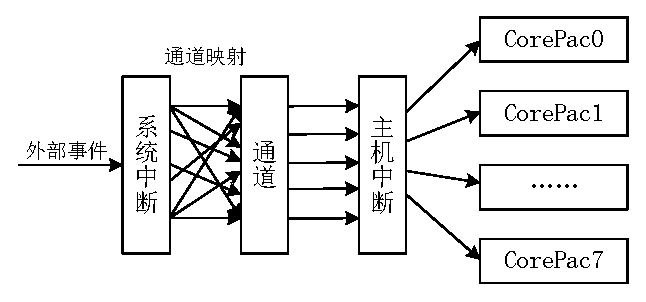
\includegraphics[width=\textwidth]{summary/1.eps}
                \caption{中断系统框图}
            \end{figure}
        \end{column}
        \end{columns}
    \end{frame}

    \begin{frame}{核内中断控制器(INTC)}
        \begin{columns}
            \begin{column}{0.5\textwidth}
                \begin{itemize}
                    \setlength{\itemsep}{0.5cm}
                    \item CPU中断0-3中除了1是NMI中断,其余都没用
                    \item CPU的可屏蔽中断只有4-15
                    \item CPU响应中断后,用户不需要手动清除核内中断的标志,但\textbf{需要手动}清除系统中断的标志(如果有使用)
                \end{itemize}
            \end{column}
            \begin{column}{0.5\textwidth}
                \begin{figure}
                    \centering
                    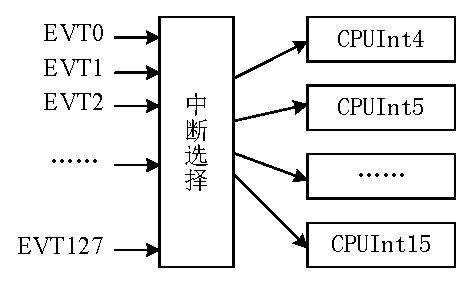
\includegraphics[width=\textwidth]{summary/2.eps}
                    \caption{核内中断控制器}
                \end{figure}
            \end{column}
        \end{columns}
    \end{frame}
    
    \begin{frame}{系统中断配置示例}
        \begin{itemize}
            \setlength{\itemsep}{0.5cm}
            \item M6678片内有一个硬件FFT模块
            \item 以FFT模块产生完成事件,触发Core0中断为例介绍配置过程
            \item M6678中断号查询.xlsx 文件可以帮助查找中断号
        \end{itemize}
        \vspace{1cm}
        \begin{figure}
            \centering
            
\includegraphics[]{summary/4.eps}
        \end{figure}
    \end{frame}

    \begin{frame}[fragile]{步骤1-确定系统中断号}
        \begin{columns}
            \begin{column}{0.5\textwidth}
                \begin{itemize}
                    \setlength{\itemsep}{0.3cm}
                    \item Core0-3由CIC0管理, Core4-7由CIC1管理
                    \item CIC0-1负责将系统事件与映射到Core0-7的INTC
                    \item CIC2-3负责将系统事件与EDMA通道绑定
                    \item 查表可知硬件FFT的系统事件编号是\textbf{7号}
                \end{itemize}
\vspace{0.5cm}

                \scriptsize
                \begin{minted}{c}
    CpIntc_clearSysInt(0, 7); // 清除7号系统事件标志
    CpIntc_enableSysInt(0, 7); // 使能7号系统事件
                \end{minted}

            \end{column}
            \begin{column}{0.5\textwidth}
                \begin{figure}
                    \centering
                    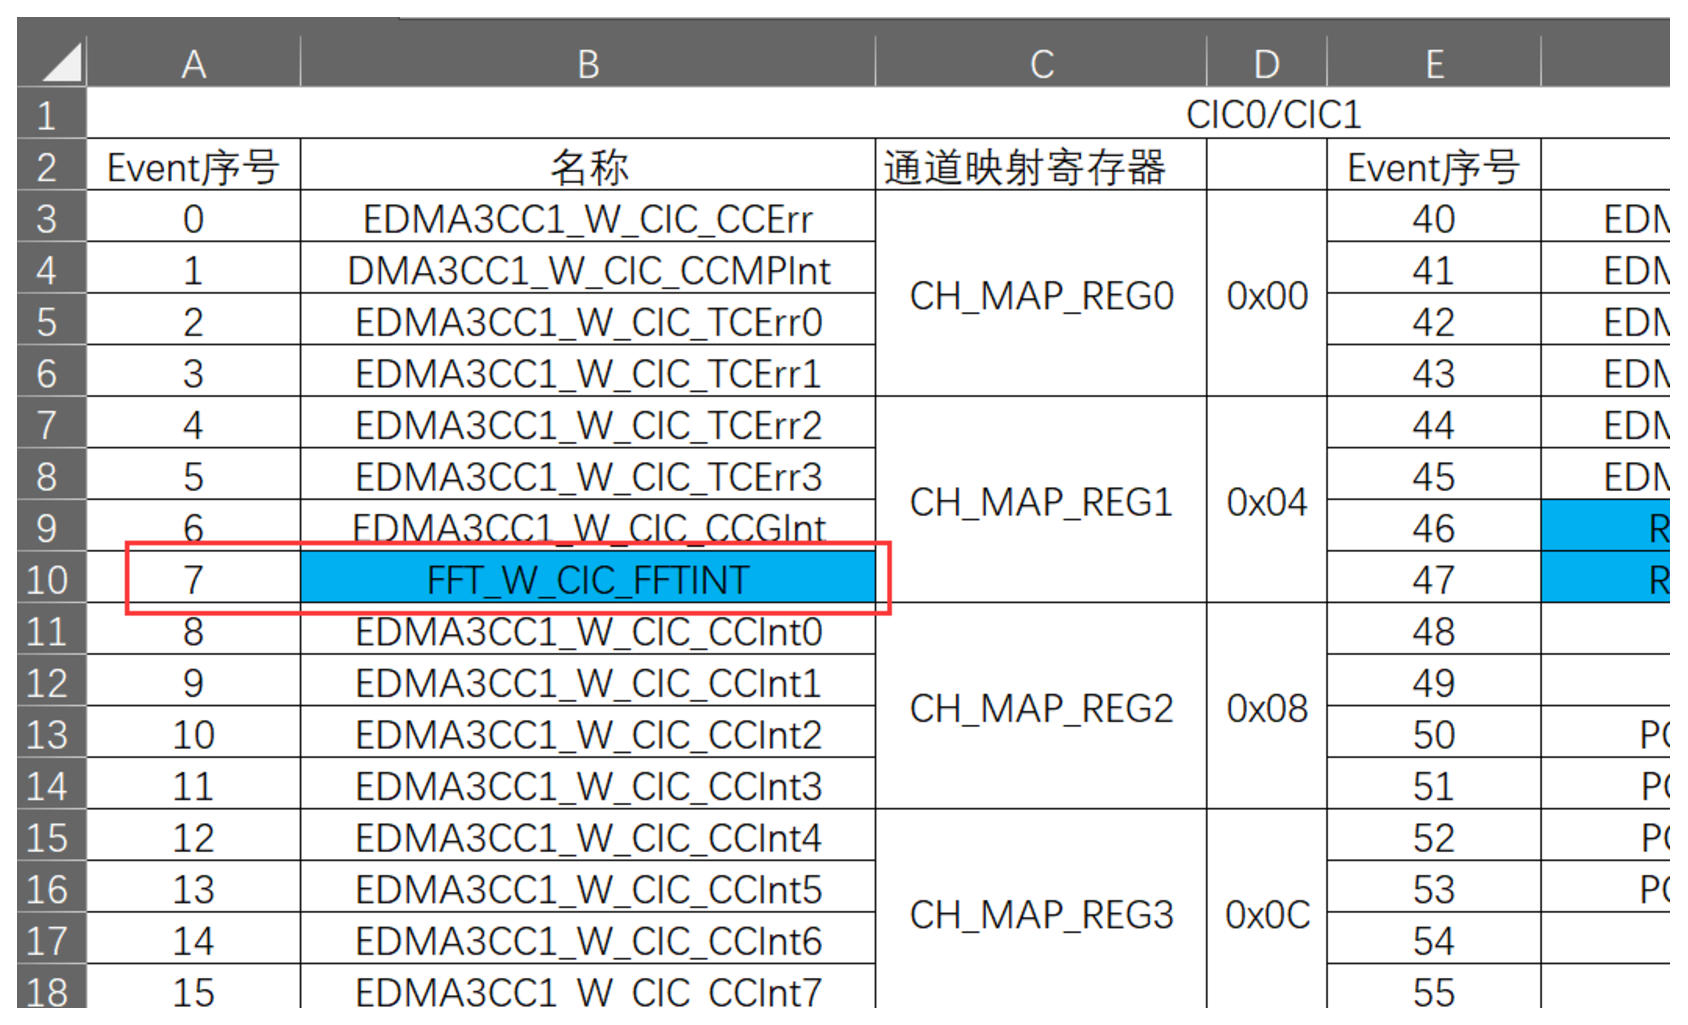
\includegraphics[width=\textwidth]{summary/3.eps}
                    \caption{系统中断号}
                \end{figure}
            \end{column}
        \end{columns}
    \end{frame}

    \begin{frame}[allowframebreaks, fragile]{步骤2-通道映射}
        \begin{figure}
        \centering
            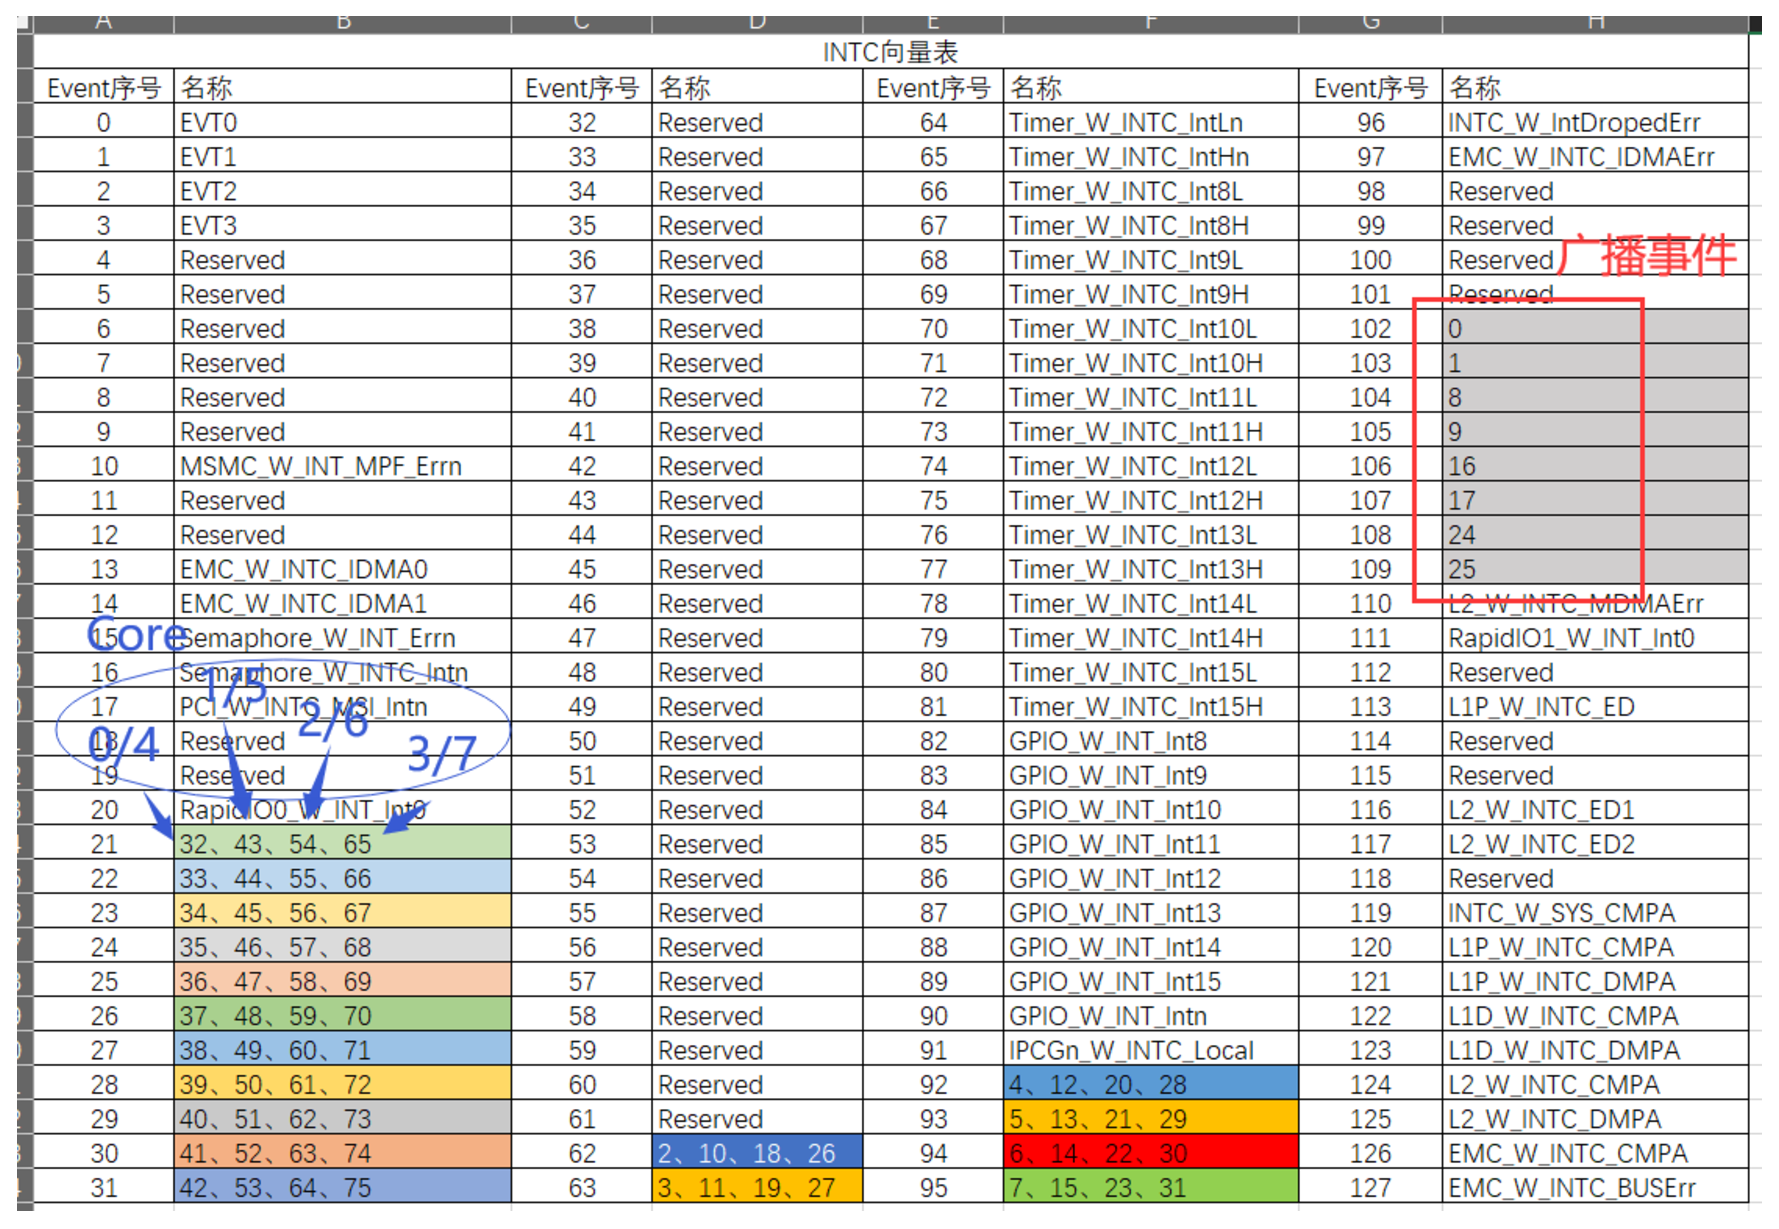
\includegraphics[width=0.8\textwidth]{summary/5.eps}
            \caption{INTC中断事件表}
        \end{figure}
        \newpage
        \begin{itemize}
            \setlength{\itemsep}{0.3cm}
            \item CIC0中的32, 43, 54, 65主机中断与Core0, Core1, Core2, Core3的21号事件绑定
            \item CIC1中的32, 43, 54, 65主机中断与Core4, Core5, Core6, Core7的21号事件绑定
            \item 0, 1, 8, ... 广播事件指的是这些主机中断每个核都能收到
            \item TIM0-7和GPIO0-7是每个核独有的中断
            \item 可以选择32号主机中断, 它和Core0的21号事件绑定
            \item 32号主机中断与32号通道绑定, 只需要把系统事件映射到32号通道即可
        \end{itemize}

        \scriptsize
        \begin{minted}{c}
    CpIntc_mapSysIntToHostInt(0, 7, 32); // 将7号系统事件与32号通道绑定
    CpIntc_enableHostInt(0, 32); // 使能32号主机中断
    CpIntc_enableAllHostInts(0); // 使能全局主机中断
        \end{minted}
    \end{frame}

    \begin{frame}[allowframebreaks, fragile]{步骤3-INTC配置}
        \begin{figure}
            \centering
            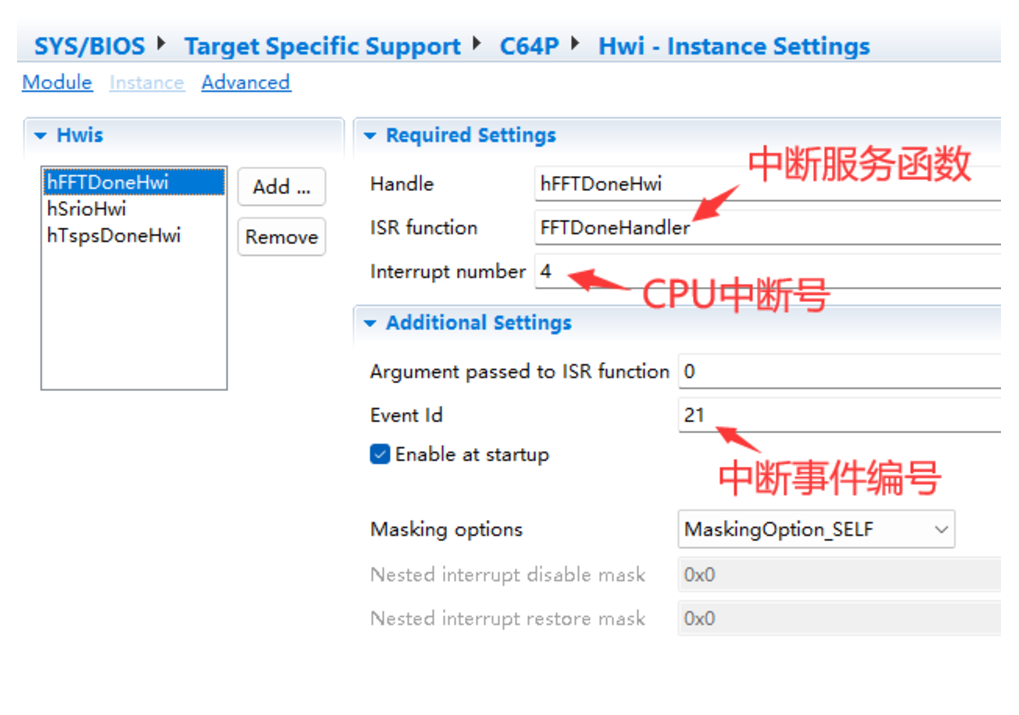
\includegraphics[width=0.8\textwidth]{summary/6.eps}
            \caption{INTC中断配置}
        \end{figure}
        \begin{itemize}
            \setlength{\itemsep}{0.3cm}
            \item Event Id 21是前面查表得到的
            \item 图中的配置是将21号事件绑定到4号CPU中断, 并且指定了中断服务函数FFTDoneHandler
        \end{itemize}
        \scriptsize
        \begin{minted}[]{c}
    /**
     * @brief 硬件FFT完成中断服务函数
     * 
     * @param a0 
     * @return Void 
     */
    Void FFTDoneHandler(UArg a0)
    {
        ......
    }
        \end{minted}
    \end{frame}

\section{EDMA的使用}

    \begin{frame}[allowframebreaks]{EDMA的组成}
    \begin{figure}
        \centering
        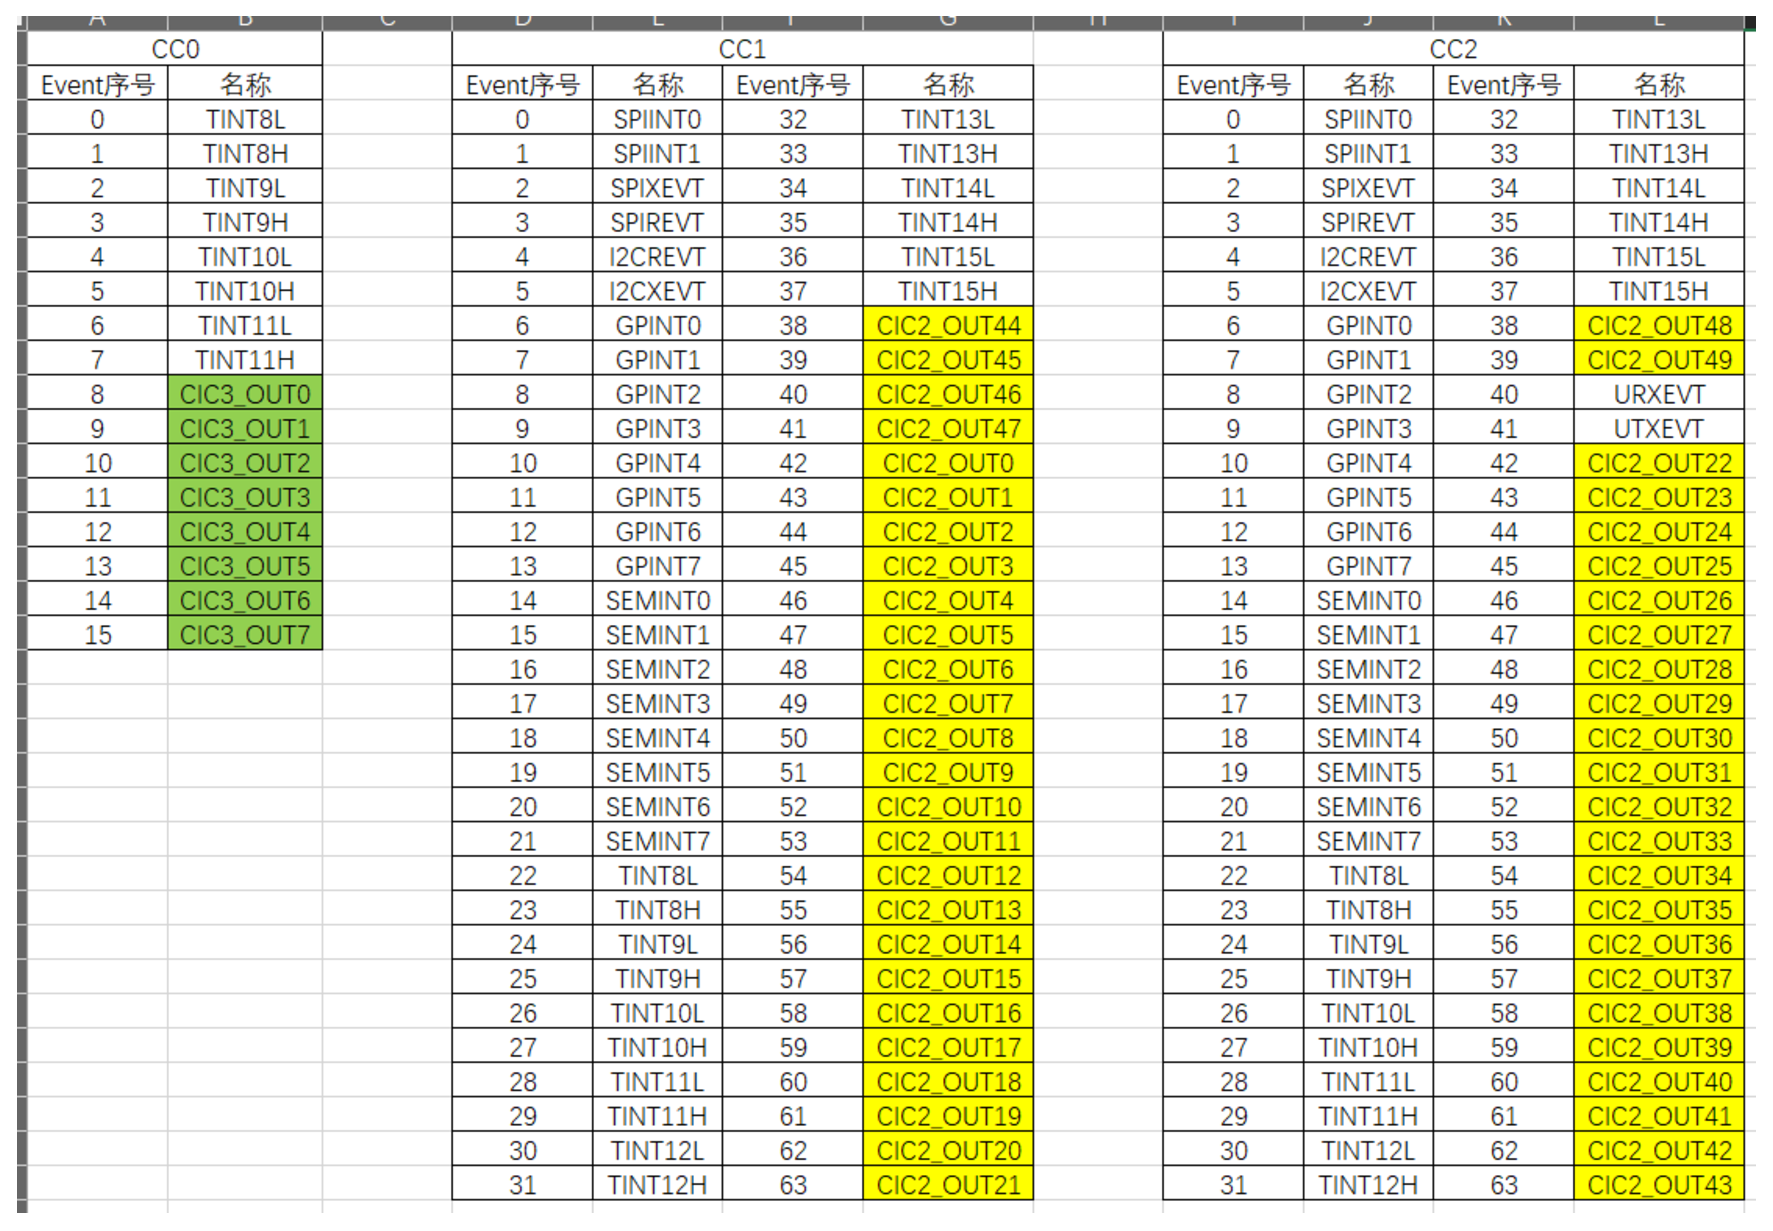
\includegraphics[width=0.8\textwidth]{summary/7.eps}
        \caption{EMDA传输控制器的通道}
    \end{figure}
    \begin{figure}
        \centering
        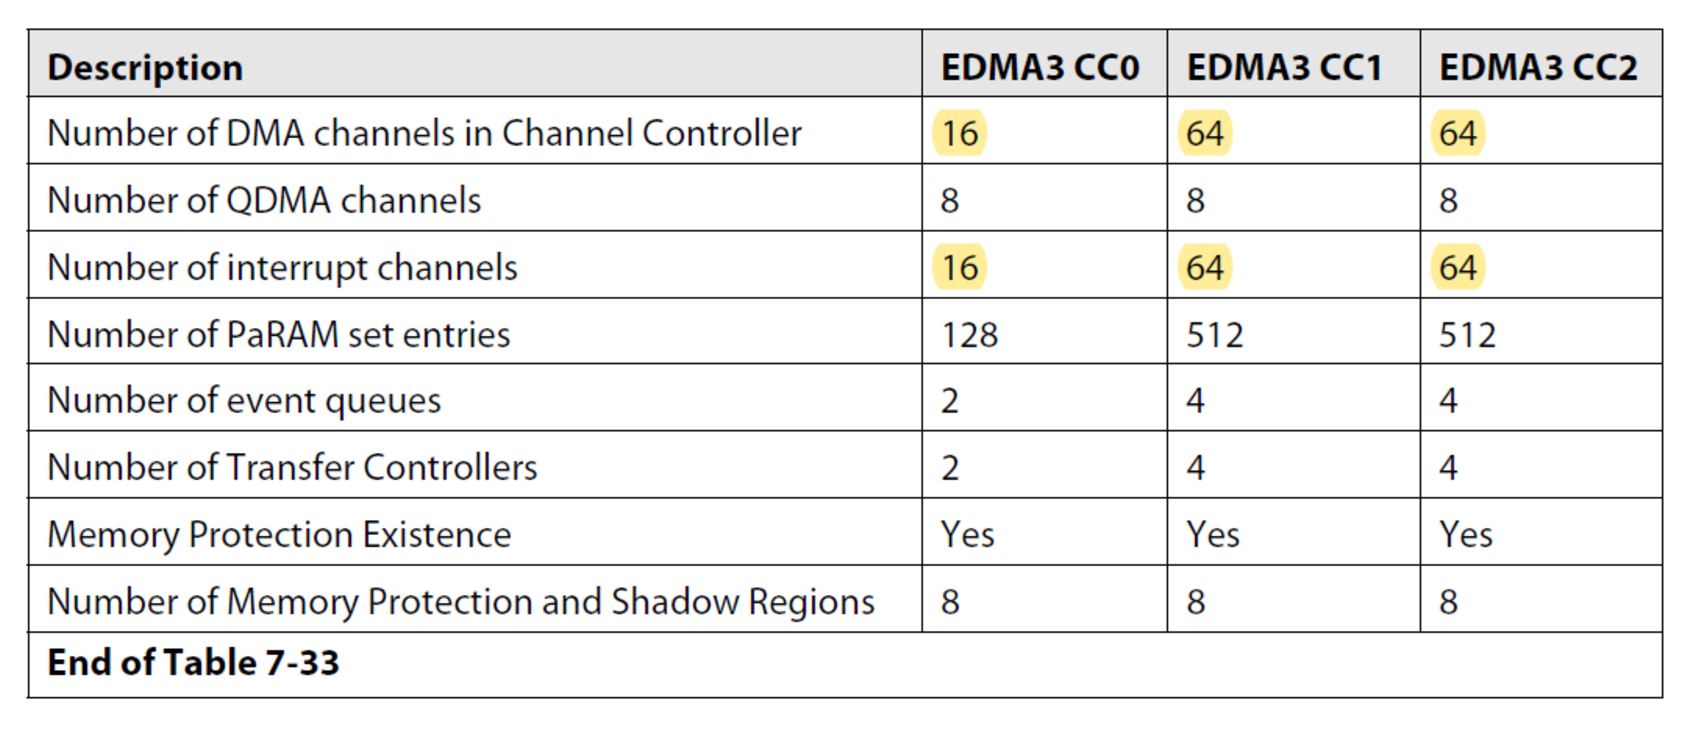
\includegraphics[width=0.7\textwidth]{summary/8.eps}
    \end{figure}
    \begin{figure}
        \centering
        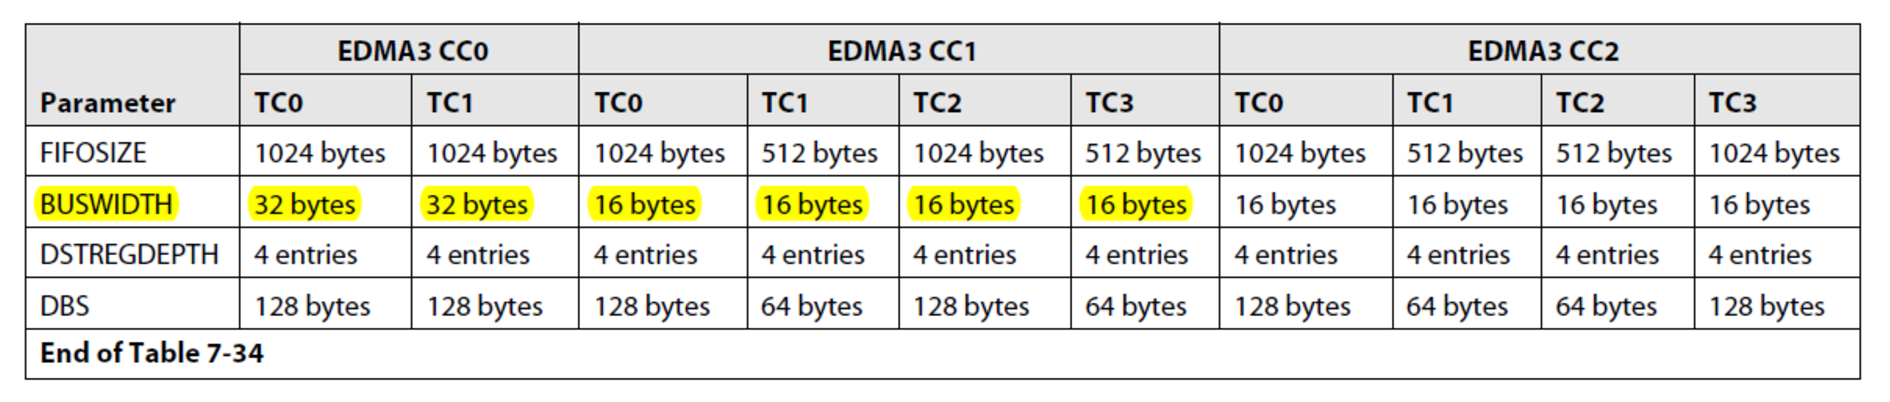
\includegraphics[width=\textwidth]{summary/9.eps}
    \end{figure}
    \begin{center}
        CC0通道数少, 但是总线位宽更宽, 会相对更快一些
    \end{center}
    \end{frame}

    \begin{frame}[allowframebreaks]{EDMA中断}
    \begin{figure}
        \centering
        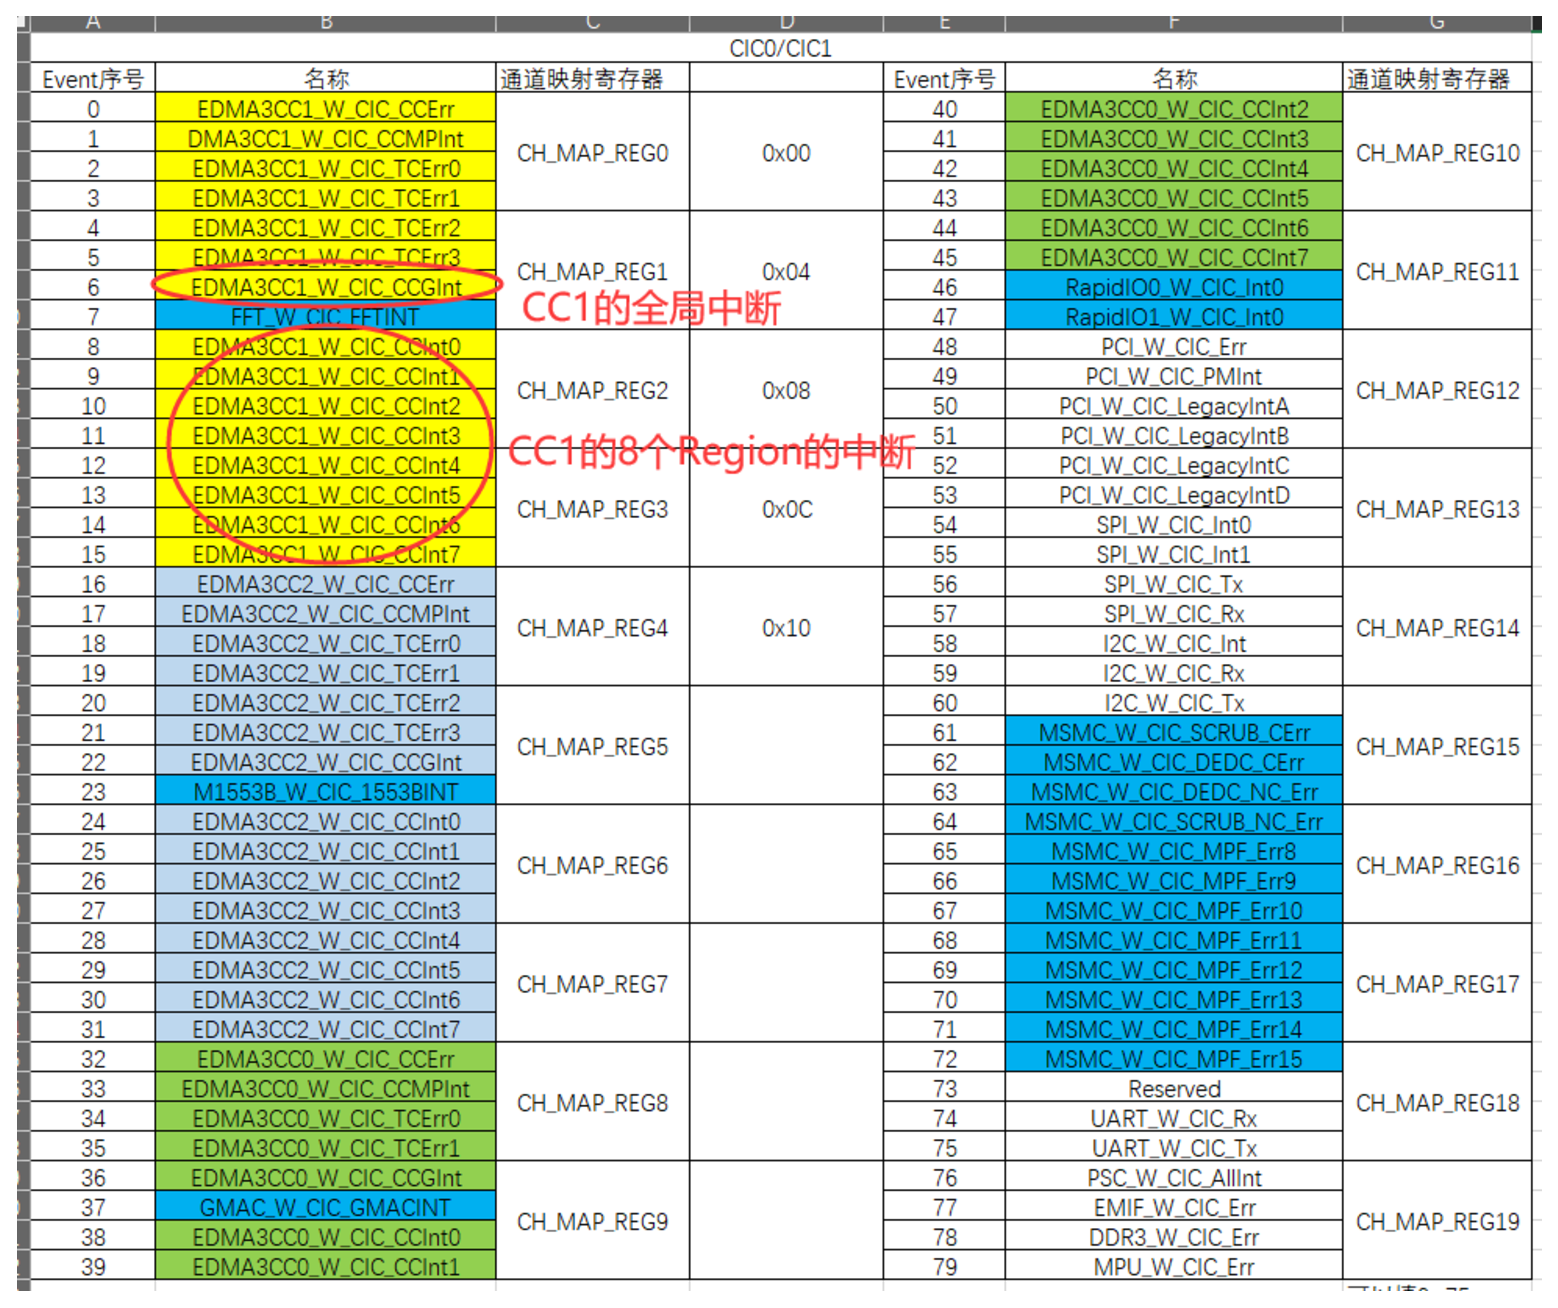
\includegraphics[width=0.8\textwidth]{summary/10.eps}
    \end{figure}
    \begin{itemize}
        \setlength{\itemsep}{0.3cm}
        \item 每个CC都有8个Region
        \item 每个Region可以使能任意的通道
        \item 某个通道产生中断时, 全局中断会产生, 使能了对应通道的Region也会产生中断
    \end{itemize}
    \end{frame}

    \begin{frame}{EDMA的PaRAM}
        \begin{figure}
            \centering
            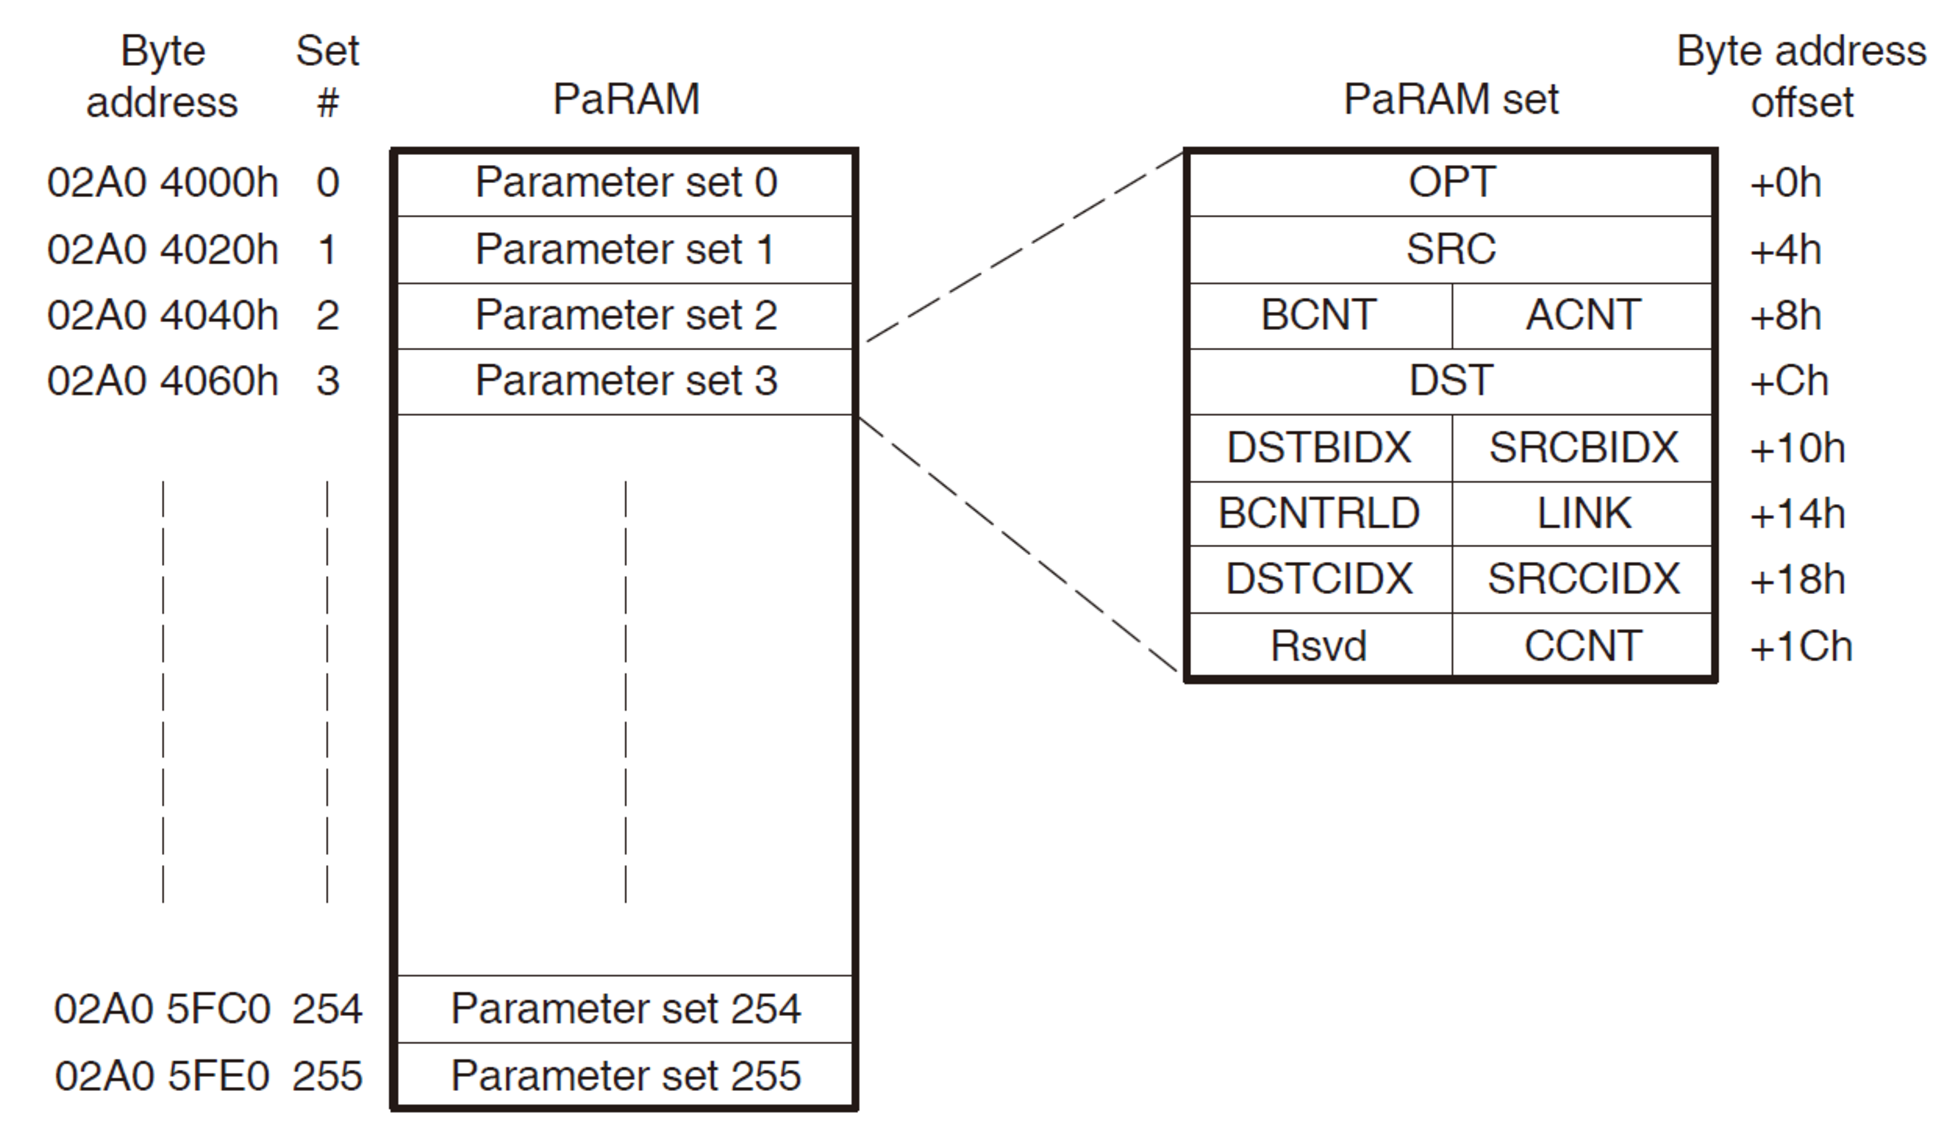
\includegraphics[width=0.8\textwidth]{summary/11.eps}
            \caption{C6455 EDMA3 Parameter RAM}
        \end{figure}
        \begin{center}
            每个PaRAM 32字节, 从0x4000开始, 用于设置EDMA的数据搬运任务
        \end{center}
    \end{frame}

    \begin{frame}[allowframebreaks]{DMA示例1——数据块传输}
        \begin{figure}
            \centering
            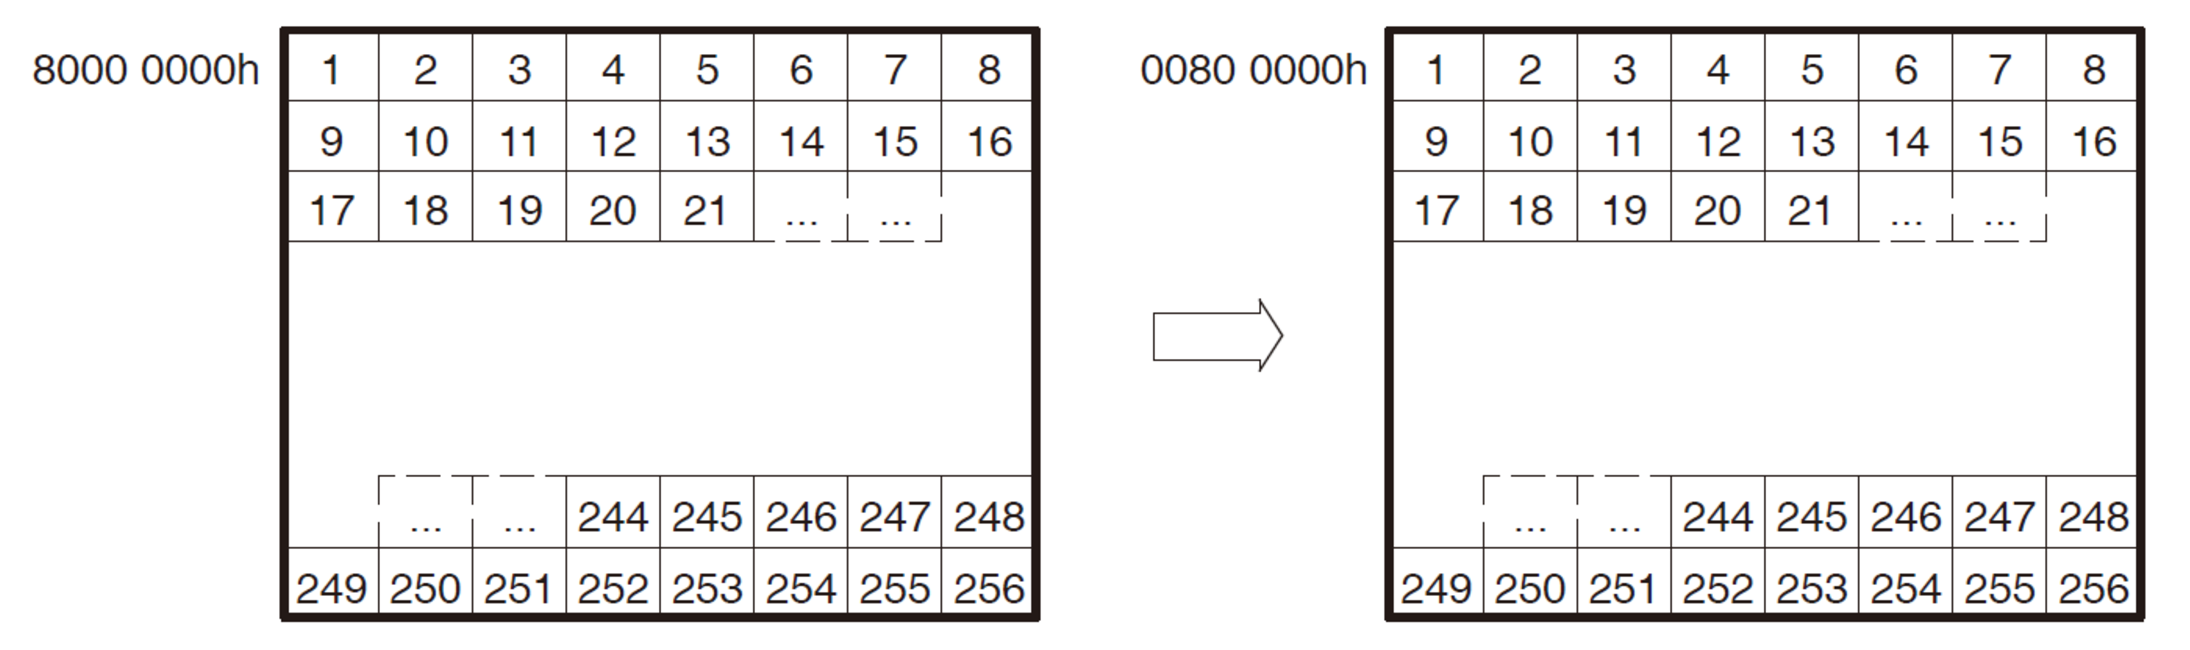
\includegraphics[width=0.9\textwidth]{summary/12.eps}
        \end{figure}
        \vspace{0.5cm}
        \begin{itemize}
            \item 从0x80000000往0x00800000传输256个Word
        \end{itemize}
        
        \begin{figure}
            \centering
            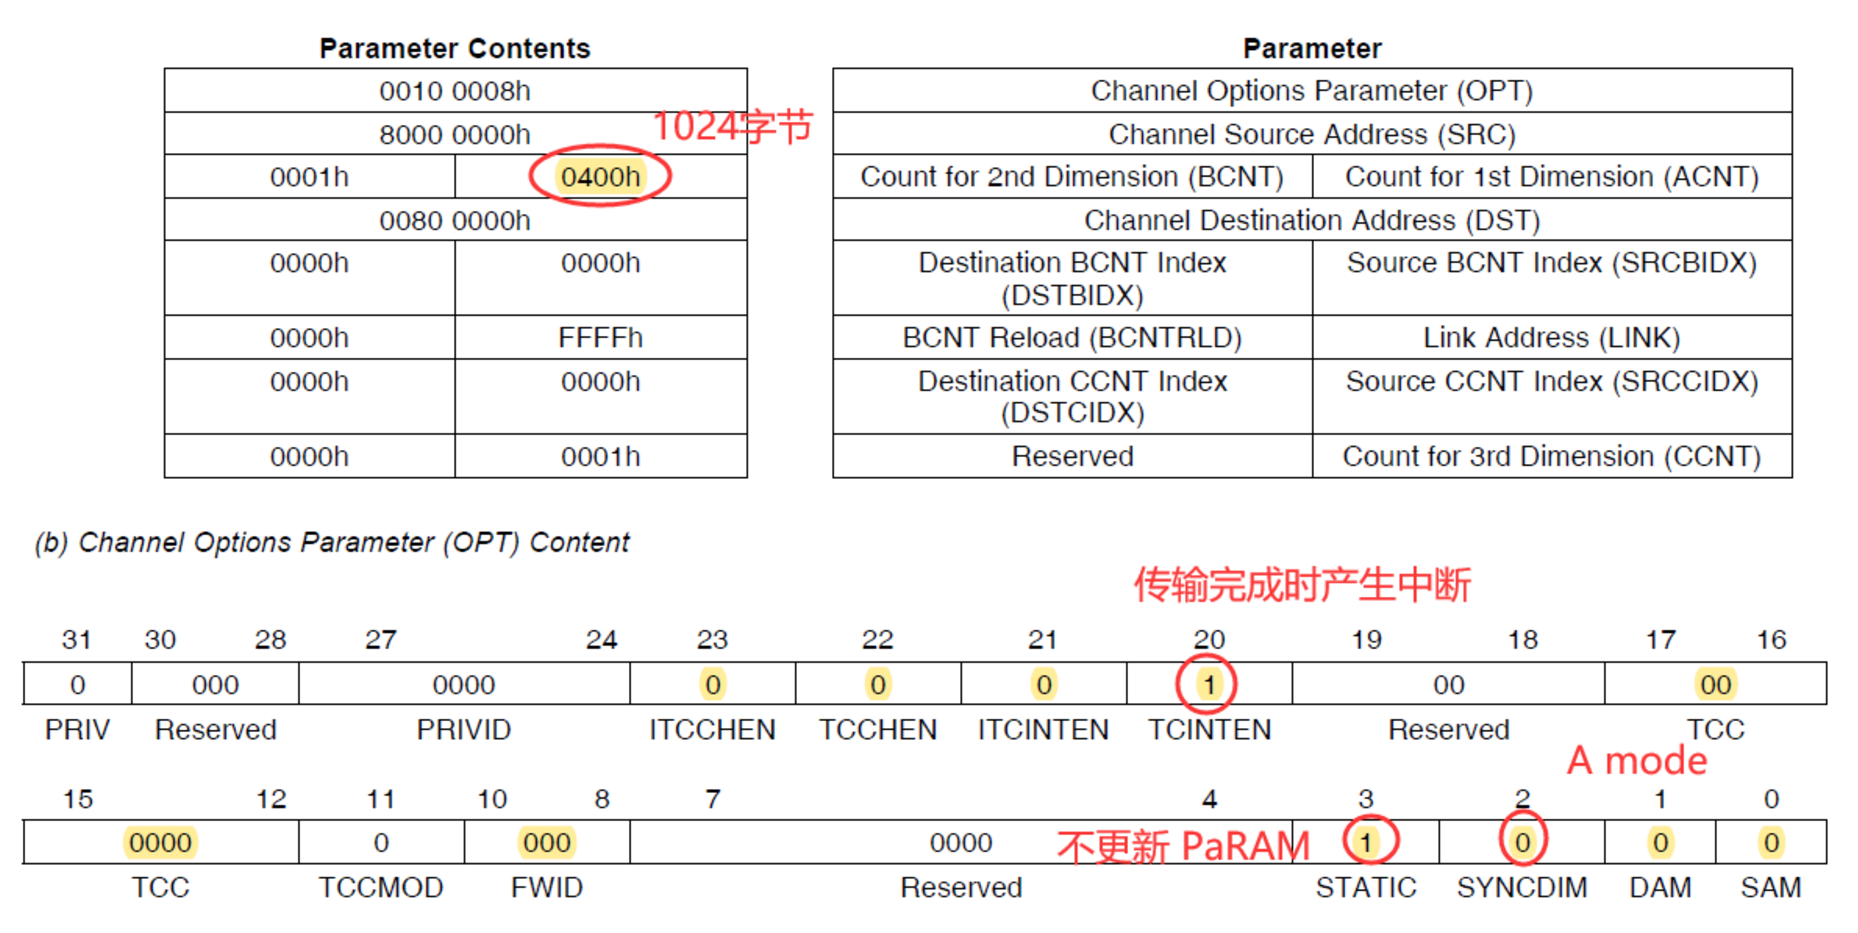
\includegraphics[width=0.9\textwidth]{summary/13.eps}
            \caption{数据块传输 PaRAM 设置}
        \end{figure}
    \end{frame}

    \begin{frame}[allowframebreaks]{DMA示例2——截取数据块}
        \begin{figure}
            \centering
            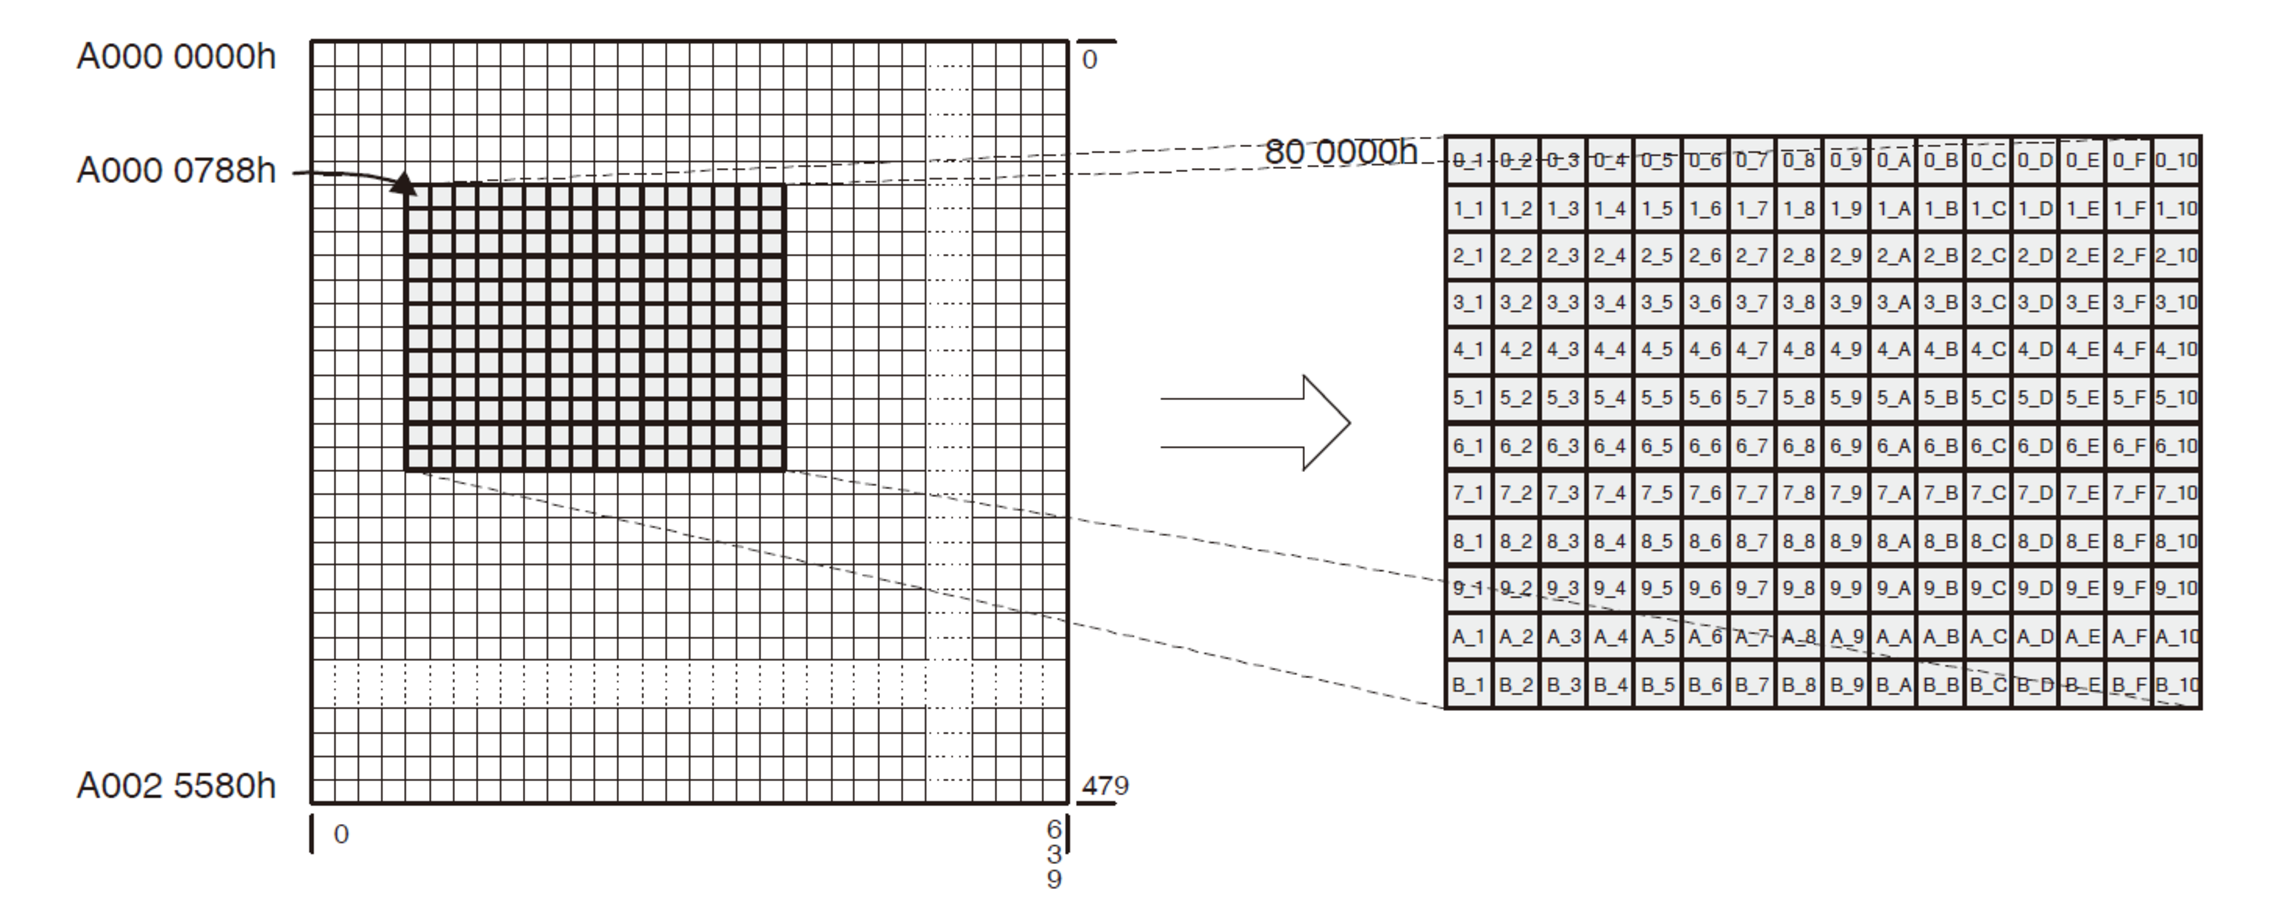
\includegraphics[width=0.9\textwidth]{summary/14.eps}
        \end{figure}
        \vspace{0.5cm}
        \begin{itemize}
            \item 从480x640的图像中截取12x16的Half Word
        \end{itemize}
        
        \begin{figure}
            \centering
            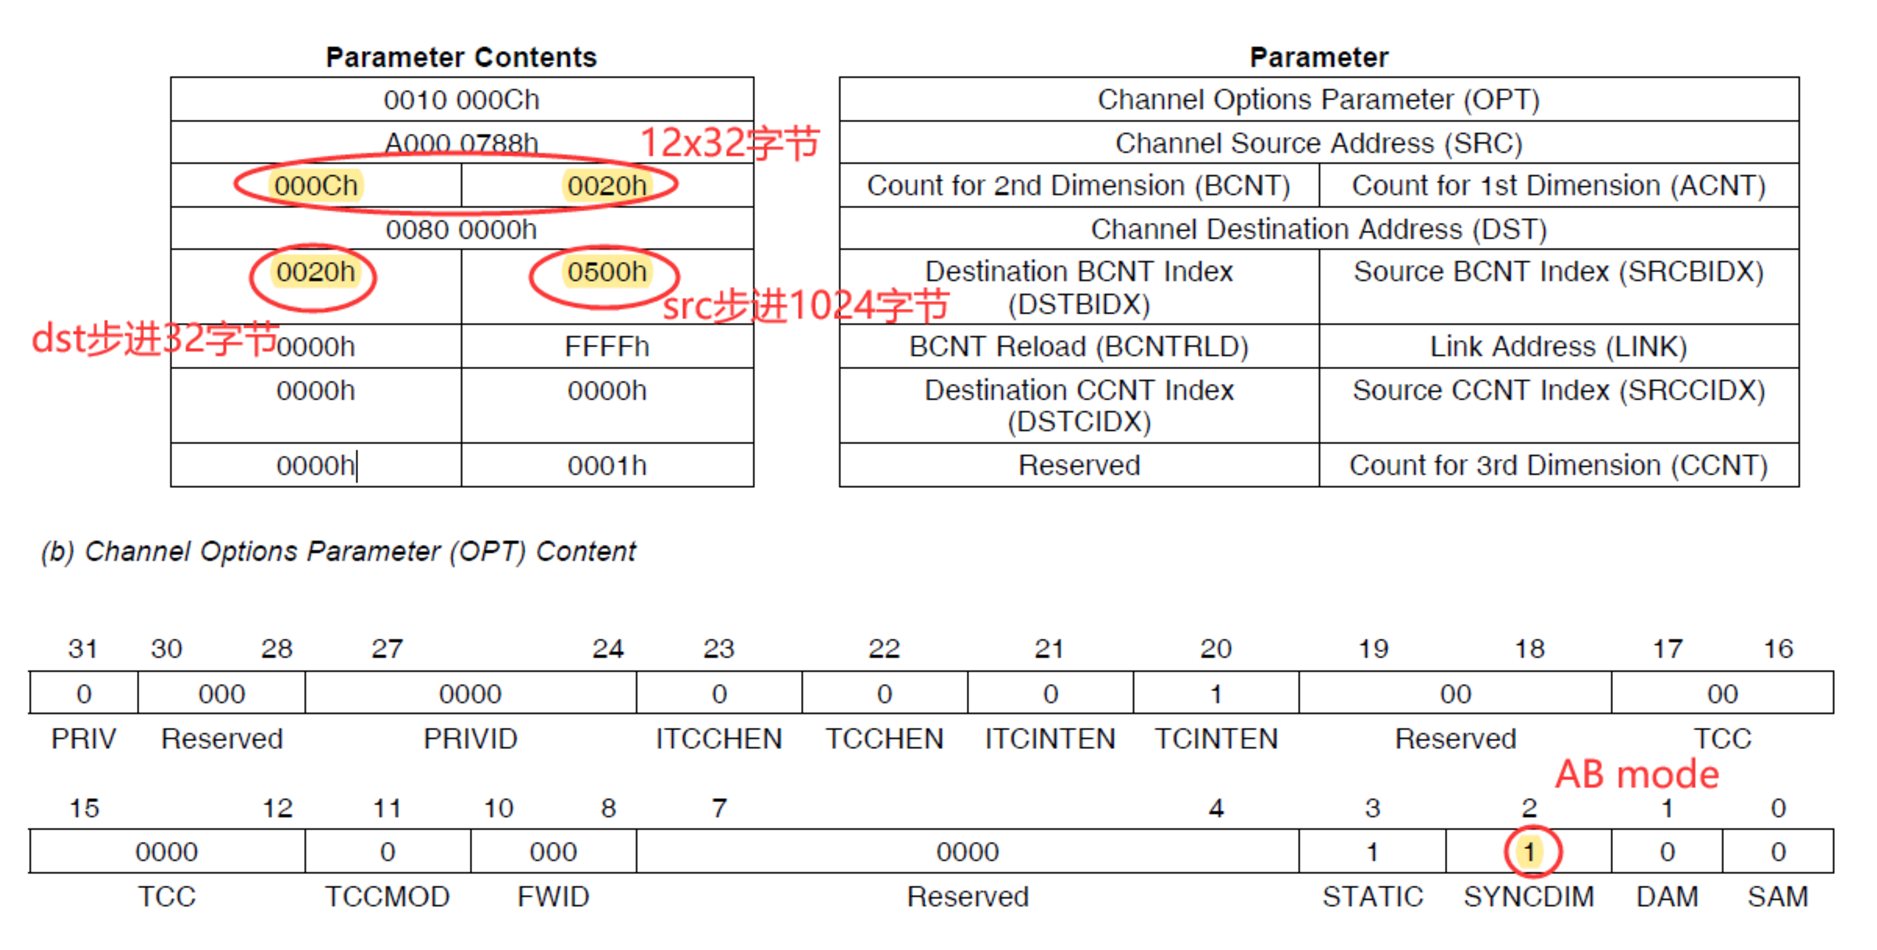
\includegraphics[width=0.9\textwidth]{summary/15.eps}
            \caption{截取数据块 PaRAM 设置}
        \end{figure}
    \end{frame}

    \begin{frame}[allowframebreaks]{DMA示例3——矩阵转置}
        \begin{figure}
            \centering
            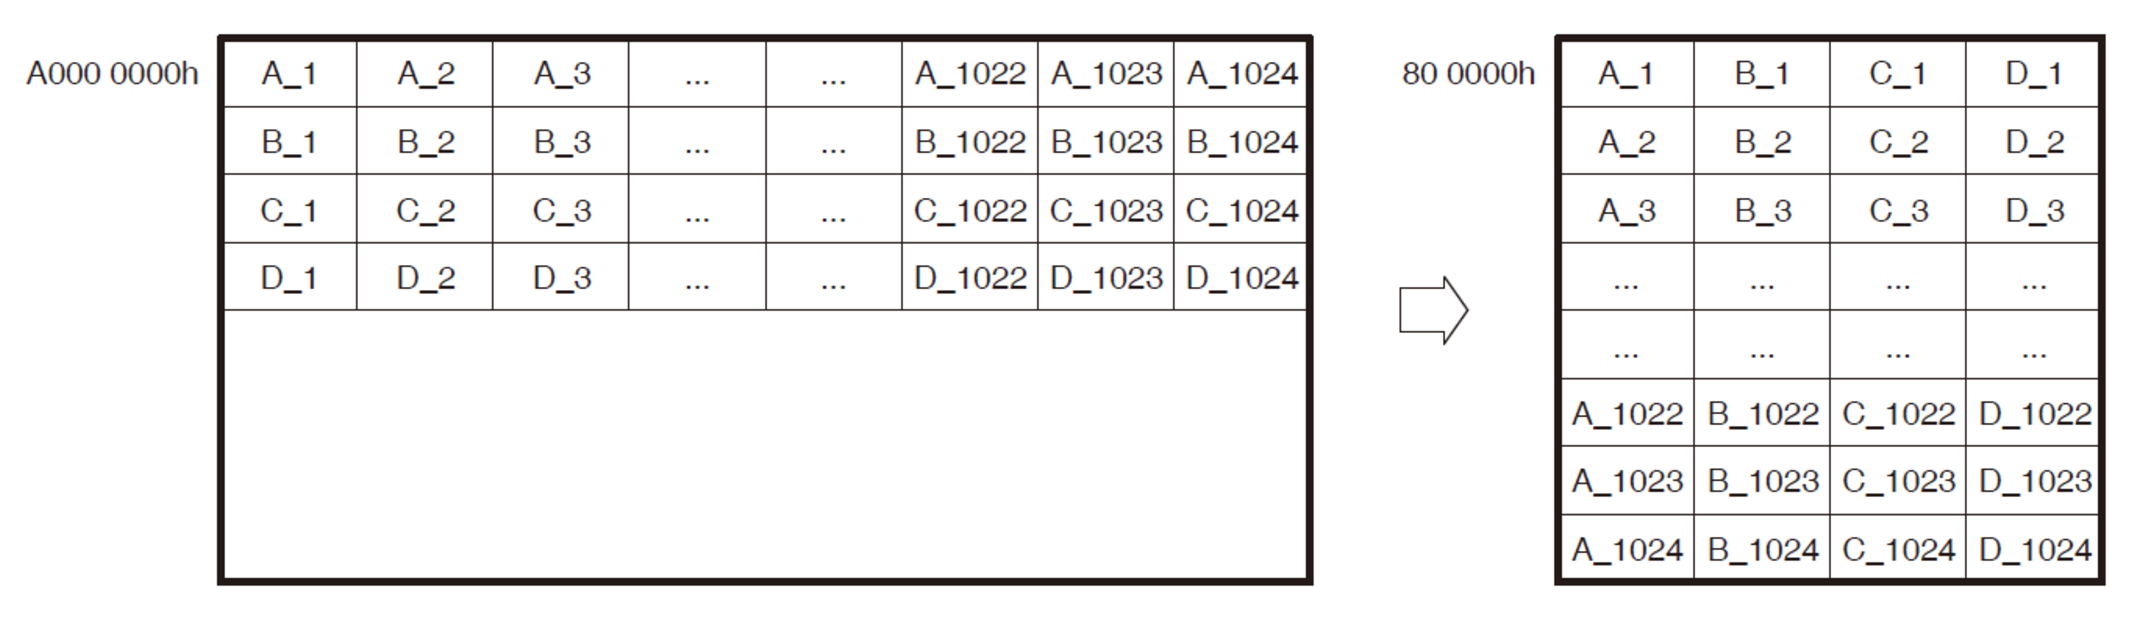
\includegraphics[width=0.9\textwidth]{summary/16.eps}
        \end{figure}
        \vspace{0.5cm}
        \begin{itemize}
            \item 将4x1024的矩阵转置, 每个数据4字节
        \end{itemize}
        
        \begin{figure}
            \centering
            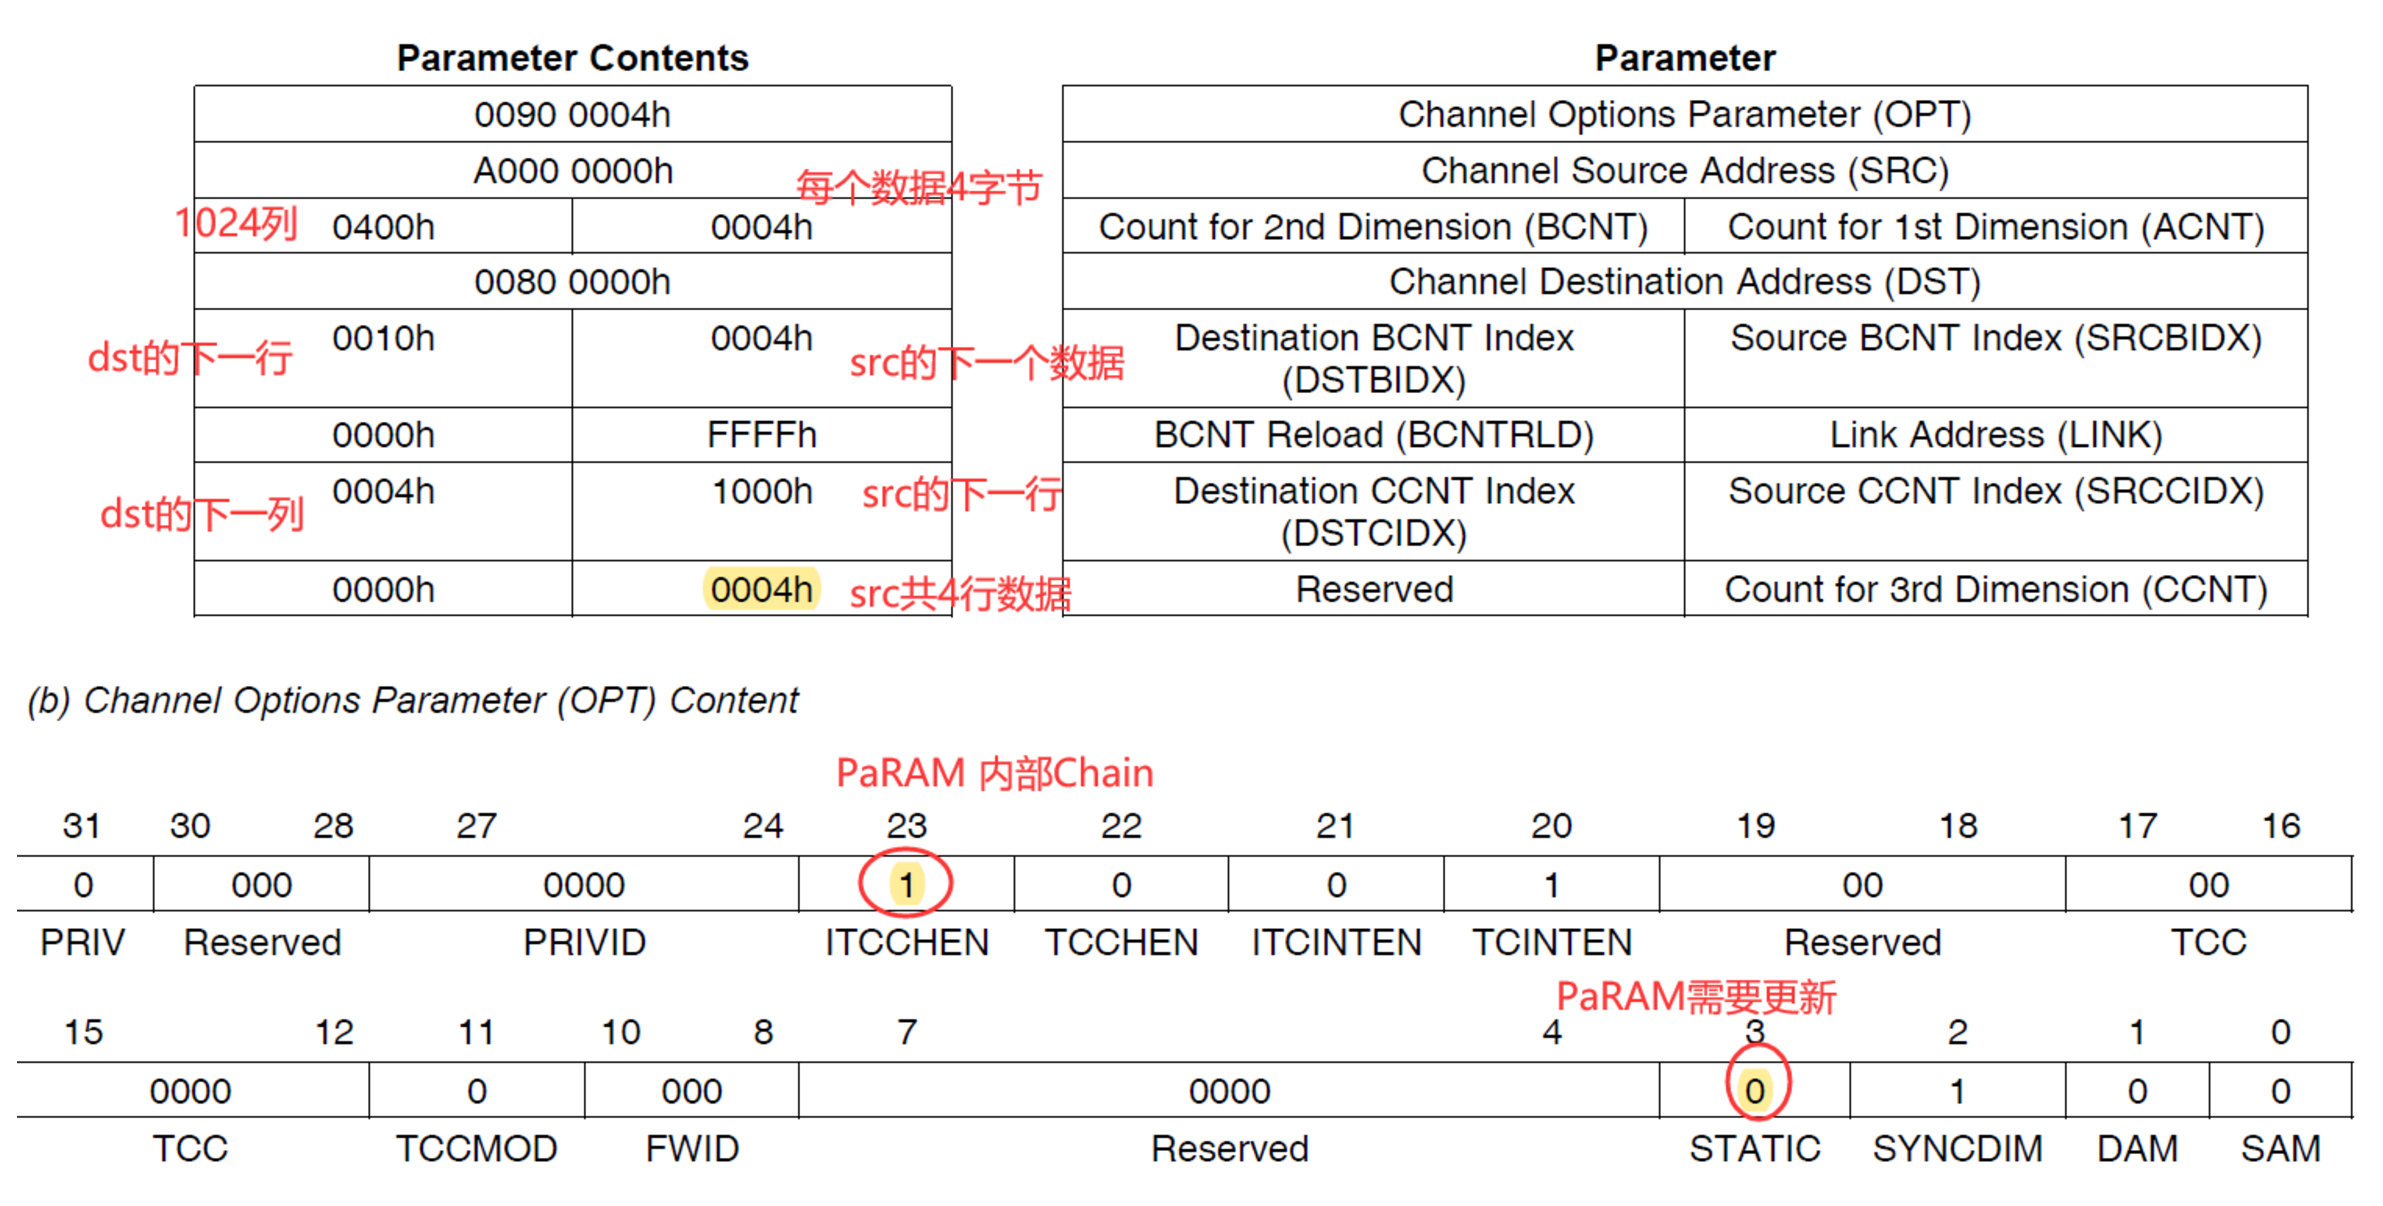
\includegraphics[width=0.9\textwidth]{summary/17.eps}
            \caption{矩阵转置 PaRAM 设置}
        \end{figure}
    \end{frame}

    \begin{frame}[allowframebreaks]{DMA示例4——McBSP数据接收}
        \begin{figure}
            \centering
            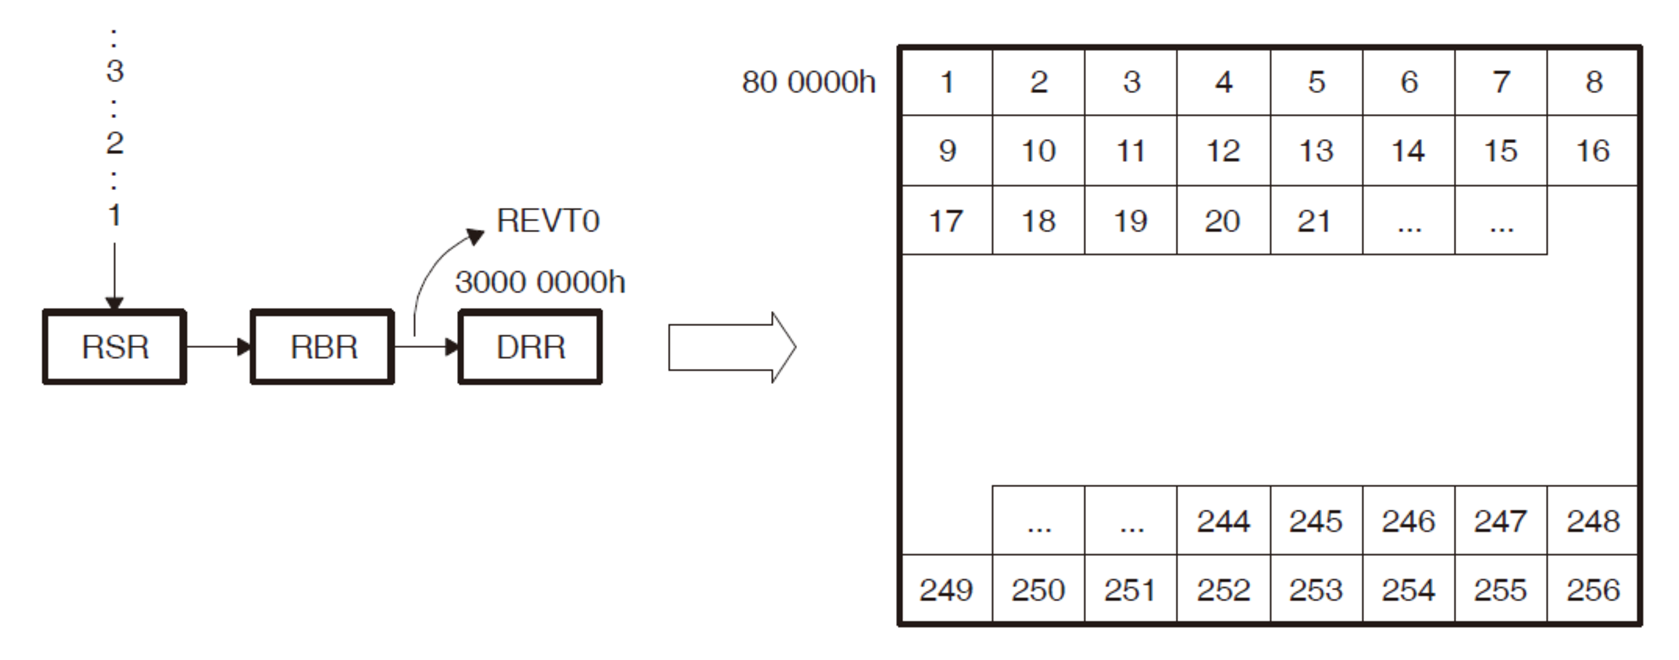
\includegraphics[width=0.9\textwidth]{summary/18.eps}
        \end{figure}
        \vspace{0.5cm}
        \begin{itemize}
            \item McBSP每接收1个Word产生一个系统中断
            \item 一帧数据256个Word, EDMA根据系统中断自动接收数据
        \end{itemize}
        
        \begin{figure}
            \centering
            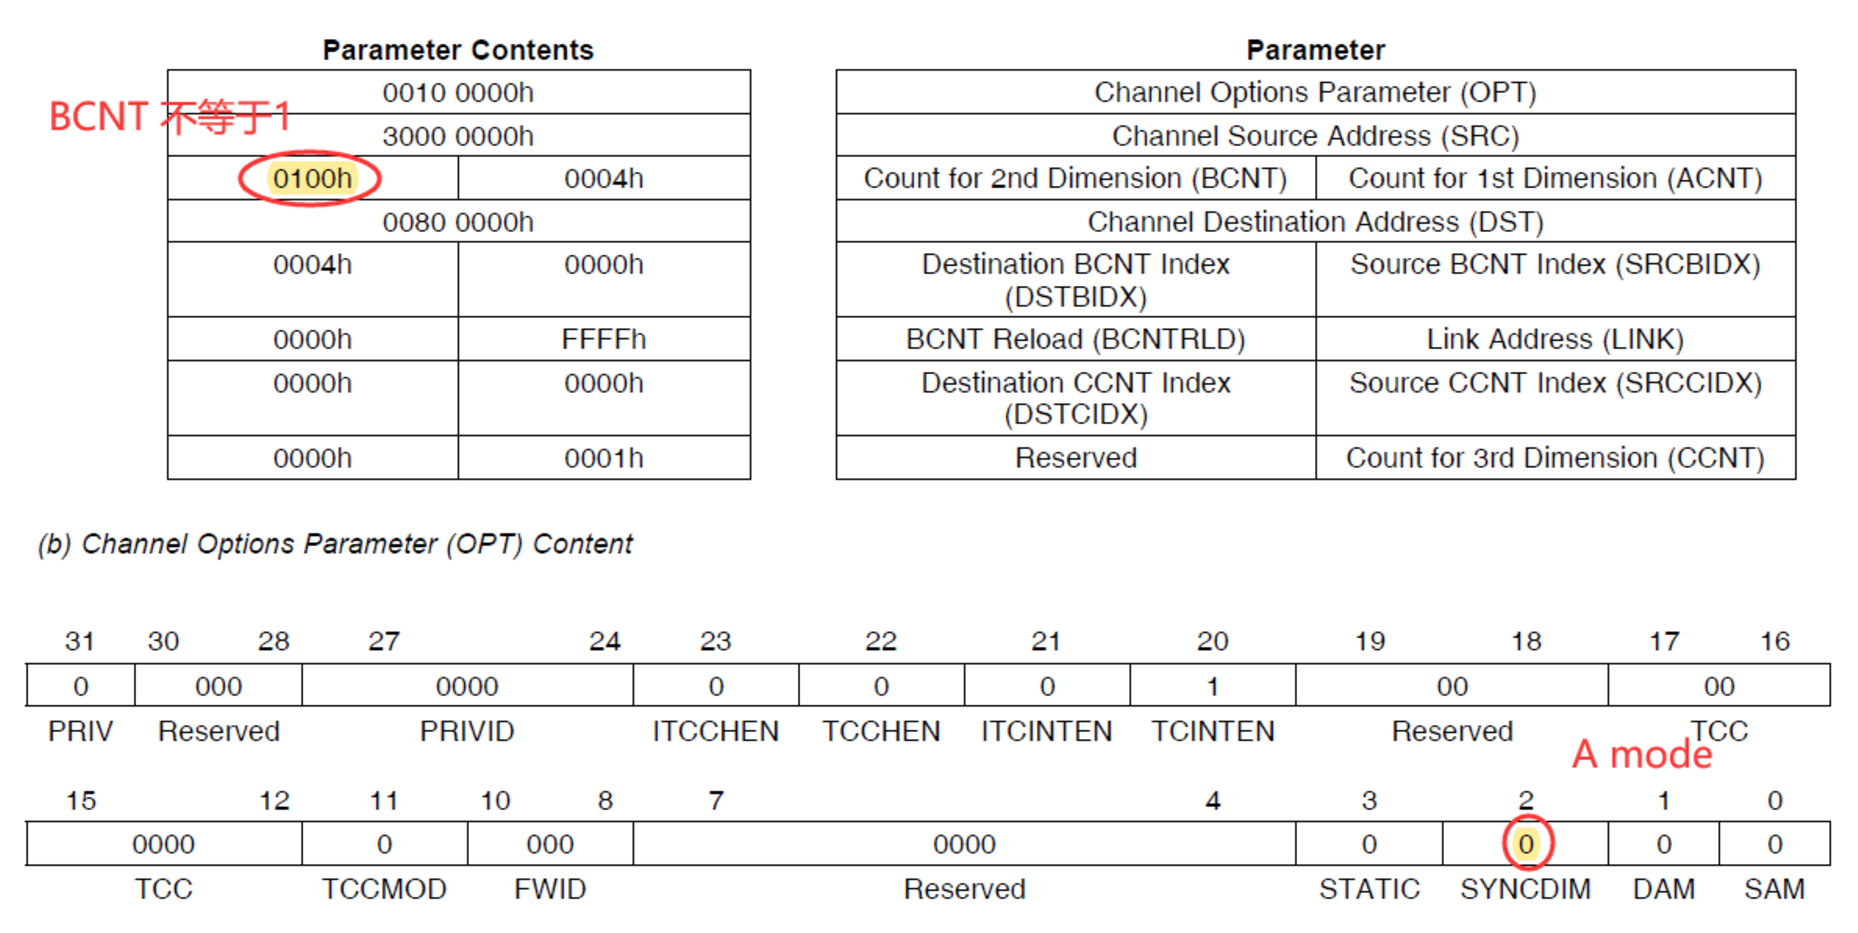
\includegraphics[width=0.9\textwidth]{summary/19.eps}
            \caption{McBSP数据接收 PaRAM 设置}
        \end{figure}
    \end{frame}

    \begin{frame}[allowframebreaks]{DMA示例5——连续数据接收}
        \begin{figure}
            \centering
            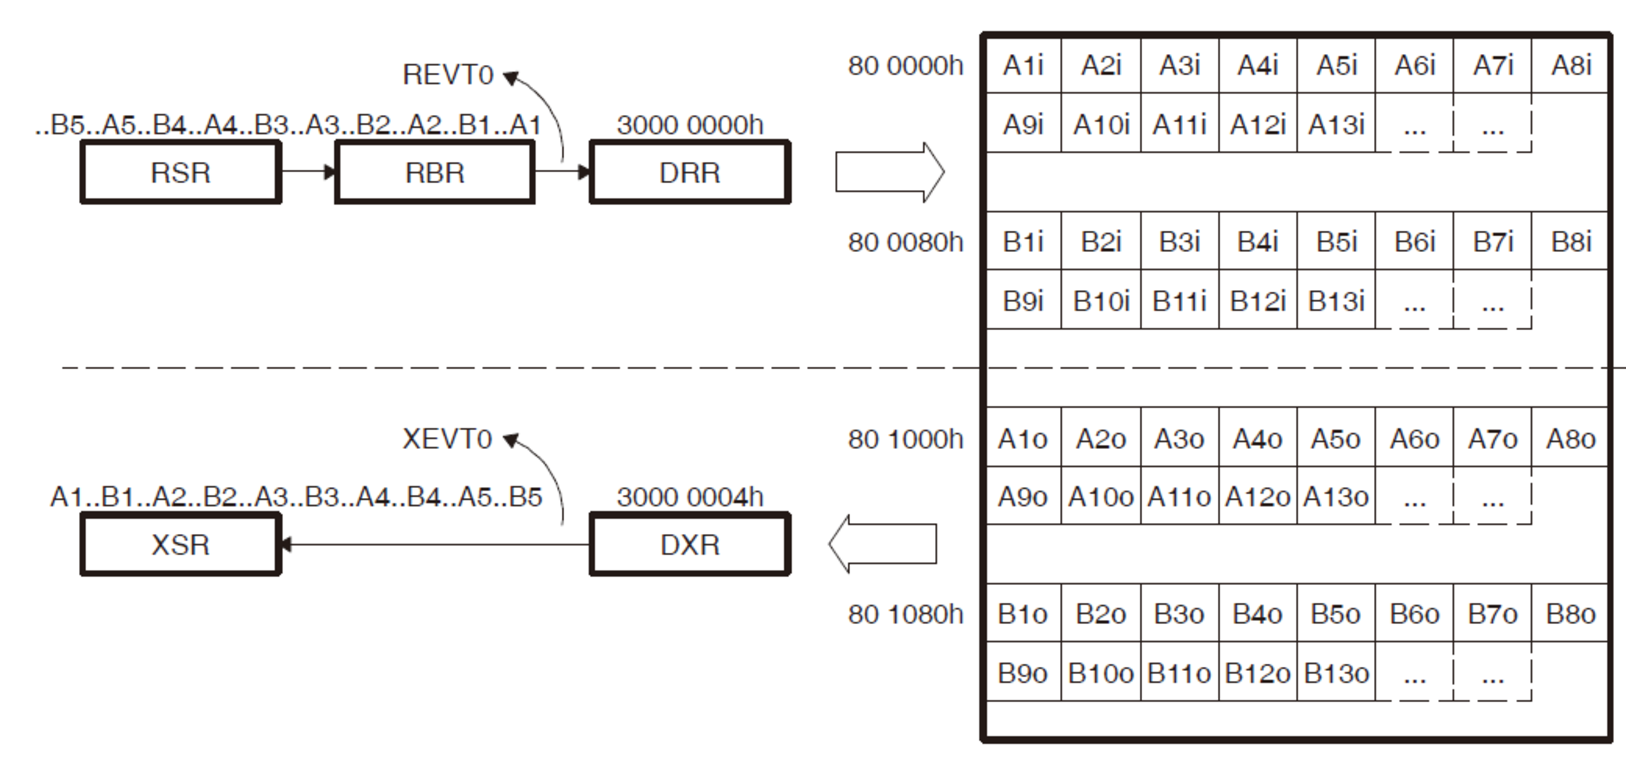
\includegraphics[width=0.9\textwidth]{summary/20.eps}
        \end{figure}
        \vspace{0.5cm}
        \begin{itemize}
            \item 一帧数据128个Word, 有连续的数据帧需要接收和发送
        \end{itemize}
        
        \begin{figure}
            \centering
            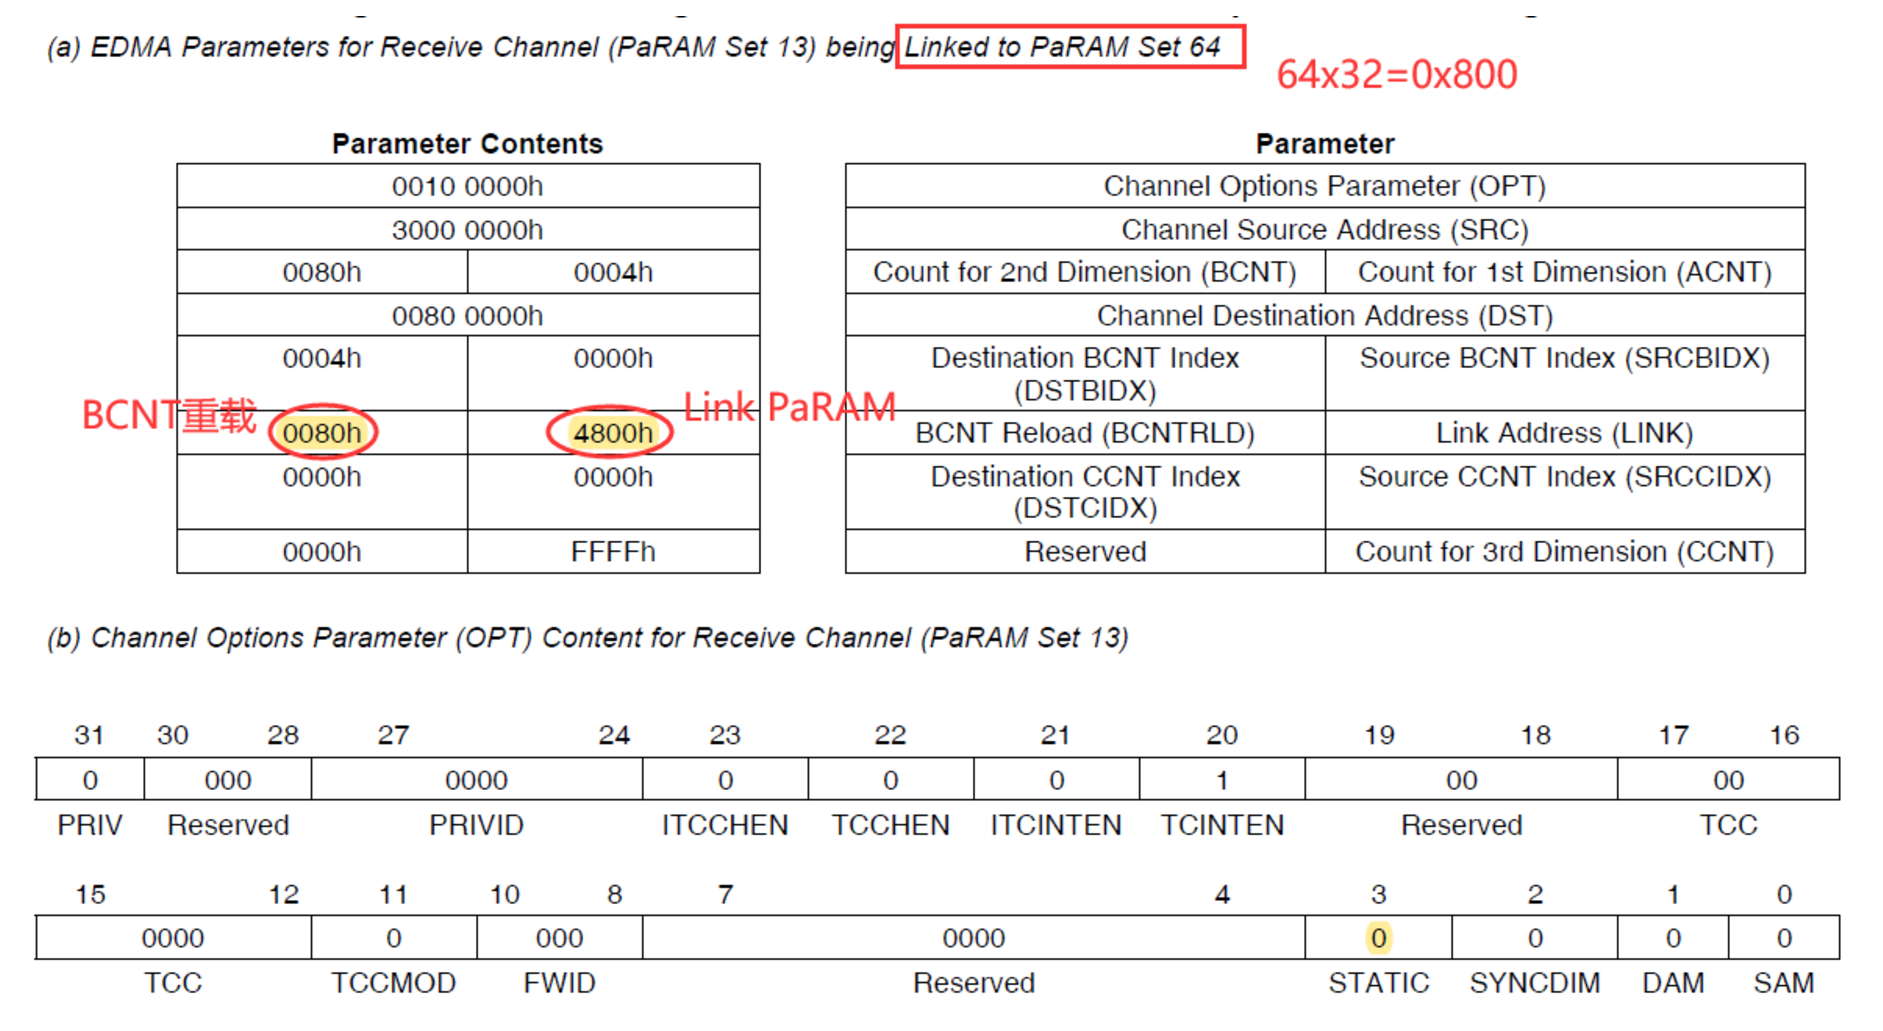
\includegraphics[width=0.9\textwidth]{summary/21.eps}
            \caption{连续数据接收 PaRAM 设置}
        \end{figure}
        \begin{itemize}
            \item PaRAM 64与PaRAM 13相同, PaRAM 13的CCNT为0时发生Link
        \end{itemize}
    \end{frame}

    \begin{frame}[allowframebreaks]{DMA示例6——Ping-Pong数据接收}
        \begin{figure}
            \centering
            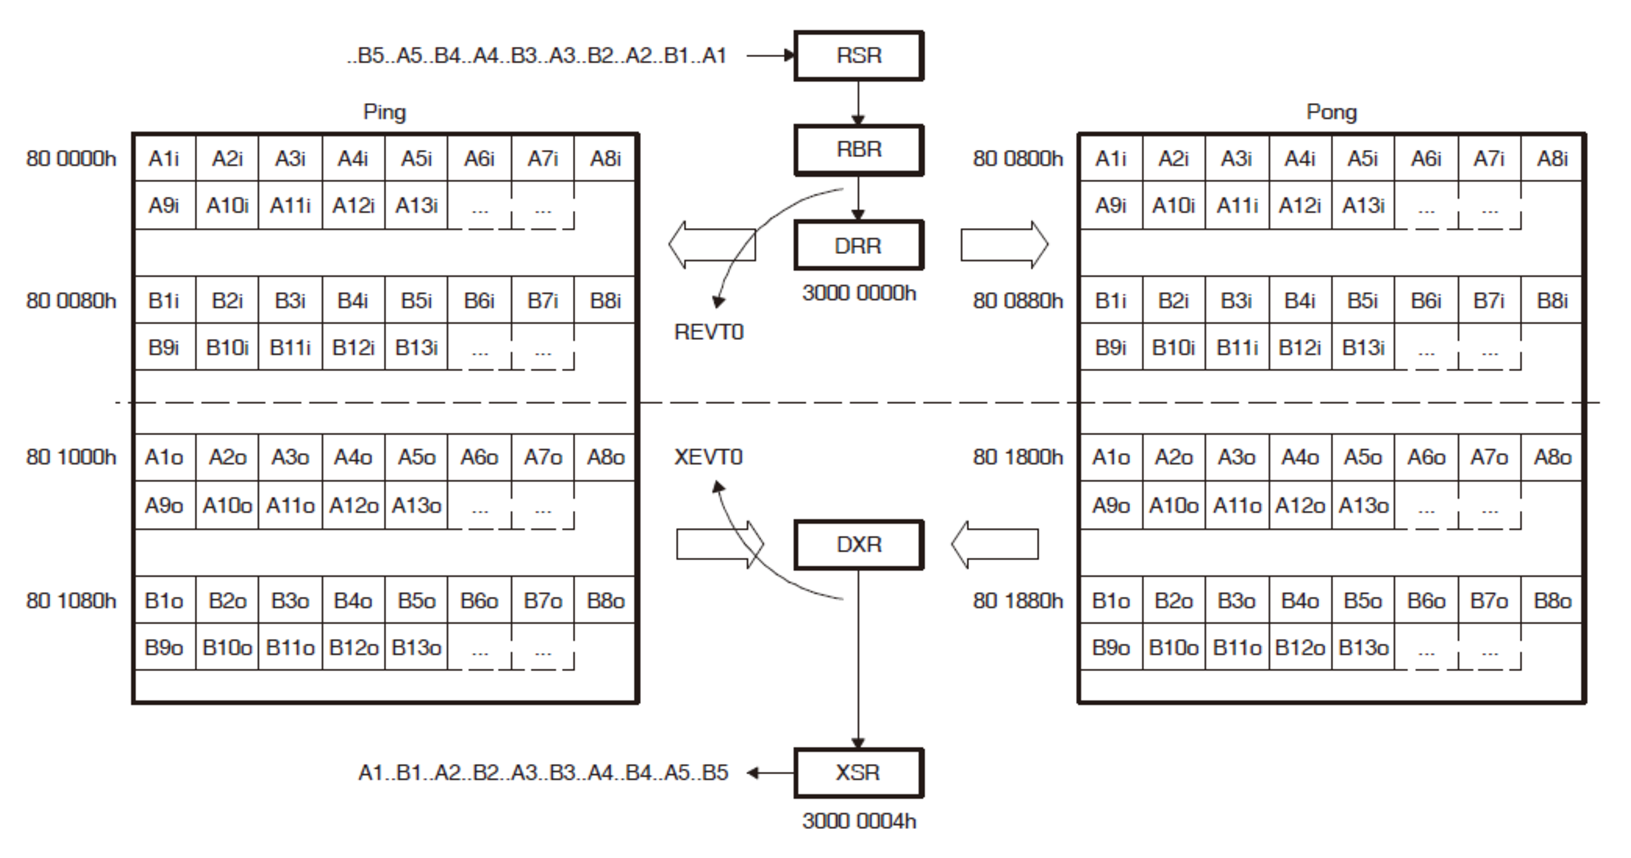
\includegraphics[width=0.9\textwidth]{summary/22.eps}
        \end{figure}
        \vspace{0.5cm}
        \begin{itemize}
            \item 一帧数据128个Word, 接收和发送缓冲区采用Ping-Pong方式
        \end{itemize}
        
        \begin{figure}
            \centering
            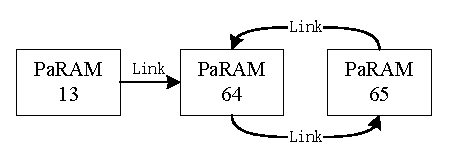
\includegraphics[width=0.7\textwidth]{summary/23.eps}
            \caption{Ping-Pong数据接收 PaRAM 设置}
        \end{figure}
        \begin{itemize}
            \item PaRAM 64和65交替Link到PaRAM 13
        \end{itemize}
    \end{frame}

\section{其它}

    \begin{frame}{其它}
    \begin{itemize}
        \setlength{\itemsep}{0.3cm}
        \item \href{https://blog.csdn.net/qq_35787848/article/details/124370431}{RTSC与XDCTools}
        \item \href{https://blog.csdn.net/qq_35787848/article/details/124988004}{OpenMP在多核DSP上的应用}
        \item \href{https://blog.csdn.net/qq_35787848/article/details/125274477}{SYS/BIOS与SRIO应用实例}
        \item \href{https://blog.csdn.net/qq_35787848/article/details/127146068}{硬件FFT加速模块的应用}
        \item \href{https://blog.csdn.net/qq_35787848/article/details/127180877}{DSP优化技术入门}
        \item \href{https://blog.csdn.net/qq_35787848/article/details/123386277}{日常总结1}
        \item \href{https://blog.csdn.net/qq_35787848/article/details/127141187}{日常总结2}
    \end{itemize}
    \end{frame}

\end{document}
